\documentclass[a4paper,10pt,titlepage]{report}
%%This template is based on Paco van Beckhoven's thesis. 

\usepackage{xspace}
\usepackage{xargs}   % Use more than one optional parameter in a new commands
\usepackage[pdftex,dvipsnames]{xcolor}

% Putting images next to each other
\usepackage[font=bf,]{caption}
\usepackage{subcaption}
\input{glyphtounicode}

% for last page
\usepackage{lastpage}

\usepackage[english]{babel}
\usepackage[utf8]{inputenc}
\usepackage{csquotes}
\usepackage[margin=1in]{geometry}
\usepackage{fancyhdr}
\usepackage{booktabs}
\usepackage{paralist}
\usepackage{graphicx}
\usepackage{tabularx}
\usepackage{adjustbox}
\usepackage{titlepic}
\usepackage{vhistory}
\usepackage{enumitem}
\usepackage{longtable}
\usepackage[backend=biber, style=ieee,citestyle=numeric-comp]{biblatex}
\usepackage[colorinlistoftodos, prependcaption]{todonotes}
\usepackage{placeins}
\usepackage{multirow}
\usepackage{amsmath,amssymb}
\usepackage[hidelinks]{hyperref}
\usepackage[acronym,nogroupskip,nohypertypes={acronym},toc,section=chapter]{glossaries}
\usepackage{amssymb}
\usepackage{verbatim}
\usepackage{cmap}
\usepackage{soul}

%\usepackage[ansinew]{inputenc}
%\usepackage[T1]{fontenc}
%\usepackage{libertine}
\input{glyphtounicode}

\pdfglyphtounicode{f_f}{FB00}
\pdfglyphtounicode{f_f_i}{FB03}
\pdfglyphtounicode{f_f_l}{FB04}
\pdfglyphtounicode{f_i}{FB01}

\pdfgentounicode=1



%Appendix package + appendix in chapter title
\usepackage[titletoc]{appendix}

\definecolor{darkbrown}{rgb}{0.4, 0.26, 0.13}
\definecolor{lightbrown}{rgb}{0.71, 0.4, 0.11}
\definecolor{BurntOrange}{rgb}{0.8, 0.33, 0.0}
\definecolor{BurntRed}{rgb}{0.5, 0.0, 0.13}
\definecolor{PineGreen}{rgb}{0.0, 0.47, 0.44}
\definecolor{MidnightBlue}{rgb}{0.1, 0.1, 0.44}
\definecolor{YellowGreen}{rgb}{0.68, 1.0, 0.18}

%for highlighting findings
\usepackage{tcolorbox}

% for highlighting code examples
\usepackage{listings}

\newcommand{\ie}{\emph{i.e.},\xspace}
\newcommand{\eg}{\emph{e.g.},\xspace}
\newcommand{\etc}{\emph{etc.}\xspace}
\newcommand{\etal}{\emph{et al.}\xspace}

\newcommand{\sig}{\gls{sig}}
\newcommand{\sigs}{\glspl{sig}}

\newcommandx{\unsure}[2][1=]{\todo[linecolor=red,backgroundcolor=red!25,bordercolor=red,#1, inline]{#2}}
\newcommandx{\discussion}[2][1=]{\todo[linecolor=red,backgroundcolor=green!25,bordercolor=red,inline,#1]{#2}}

\newcommandx{\improvement}[2][1=]{\todo[linecolor=blue,backgroundcolor=blue!25,bordercolor=blue,#1]{#2}}

\newcommandx{\reminder}[2][1=]{\todo[linecolor=yellow,backgroundcolor=yellow!25,bordercolor=yellow,#1]{#2}}

\newcommandx{\lessprio}[2][1=]{\todo[linecolor=Plum,backgroundcolor=Plum!25,bordercolor=Plum,#1]{#2}}
\newcommandx{\todocontent}[2][1=]{\todo[author=\textbf{Planned content},backgroundcolor=Goldenrod!25,bordercolor=Goldenrod,inline,#1]{#2}}


%%Some additional table column specifiers, allowing for fixed width columns that wrap.
\newcolumntype{L}[1]{>{\raggedright\let\newline\\\arraybackslash\hspace{0pt}}p{#1}}
\newcolumntype{C}[1]{>{\centering\let\newline\\\arraybackslash\hspace{0pt}}p{#1}}
\newcolumntype{R}[1]{>{\raggedleft\let\newline\\\arraybackslash\hspace{0pt}}p{#1}}

\definecolor{ryel}{HTML}{fcd116}
\definecolor{rred}{HTML}{ce1126}
\definecolor{rblu}{HTML}{0a3eb9}
%these are examples of commands that may facilitate feedback annotations in the document
%replace \paco by your name and \ana by your supervisor's name
%\newcommandx{\ana}[2][1=]{\todo[linecolor=rblu,backgroundcolor=ryel,bordercolor=rred,#1]{#2}}
%\newcommandx{\paco}[2][1=]{\todo[author=Paco,linecolor=blue,backgroundcolor=white,bordercolor=red,#1]{#2}}


% -- title page is a modified version of https://github.com/software-engineering-amsterdam/latex/blob/master/thesis/uvamscse.cls
\newcommand{\email}[1]{\ttfamily\href{mailto:#1}{#1}}

\newcommand{\uvacoverfoot}{%
	\vfill
	\begin{center}
		\begin{tabular}{r|l}
			\multirow{3}{*}{
\includegraphics[height=48pt]{uva.pdf}}
			&\textsc{\Large Universiteit van Amsterdam}\\
			&\textsc{Faculteit der Natuurwetenschappen, Wiskunde en Informatica}\\
			&\textsc{Master Software Engineering}\\
			&\url{http://www.software-engineering-amsterdam.nl}
		\end{tabular}
	\end{center}
}

\renewcommand{\maketitle}{%
	% The cover page
	% --------------
	\thispagestyle{empty}
	\enlargethispage{30pt}
	\renewcommand{\thefootnote}{\fnsymbol{footnote}}
	% Will be page 0, s.t. contents start on page 1
	\setcounter{page}{0}
	% \eccoverhead
	% Volume and article title, author(s)
	\vspace{60pt}
	\begin{center}
		{\Huge\bfseries ScriptButler: Leveraging Meta-programming Principles to Facilitate the Software Evolution of Digital Games \par}
		
		\vspace{44pt}
		{\Large\bfseries Clement Julia \par}
		\email{clement.julia@student.uva.nl}\\
		\vspace{11pt}
		January 31, 2022, \pageref{LastPage} pages
	\end{center}
	\vfill
	\begin{tabular}{p{0.35\linewidth} p{0.6\linewidth}}
		\textbf{Academic supervisor:} 	& Riemer van Rozen, \email{R.A.van.Rozen@cwi.nl} \\
		\textbf{Second Reader:} 	& Ana Oprescu, \email{a.m.oprescu@uva.nl} \\
		\textbf{Third Reader:} 	& Anders Bouwer, \email{a.j.bouwer@hva.nl} \\
% 		\textbf{Daily supervisor:} & Name industry/daily supervisor, \email{industry supervisor email}\\
		\textbf{Research group:} & Centrum Wiskunde \& Informatica, Software Analysis \& Transformation, \url{https://www.cwi.nl/research/groups/software-analysis-and-transformation}
	\end{tabular}
	\uvacoverfoot
	\newpage
	\setcounter{footnote}{0}
	\renewcommand{\thefootnote}{\arabic{footnote}}
	\setlength{\parskip}{0pt}
}

%\newcommand{\uvaabstract}{}latex 
%\renewcommand{\abstract}[2][Abstract]{\renewcommand{\uvaabstract}{\chapter*{Abstract}%
%\par#2\newpage}}


%-------- End of ``title page''

%Fancy page headers
\pagestyle{fancy}
\fancyhf{}
\fancyhead[L]{\leftmark}
\fancyfoot[C]{\thepage}
\setlength{\headheight}{14pt}


%%FINDING ENV
\newcounter{findingctr}

\newenvironment{finding}{%      define a custom environment
	\refstepcounter{findingctr}% increment the environment's counter
	\begin{tcolorbox}
	\textbf{Finding \thefindingctr:}
}{\end{tcolorbox}} 
% If you want numbers that start with the chapter or section number (e.g. 7.1.1 or 7.1) enable the following lines 
%\usepackage{amsmath}
%\numberwithin{findingctr}{chapter}


% Decrease the size of all these lists
\setlist{noitemsep,topsep=4pt,parsep=1pt,partopsep=4pt}


\lstset{
	basicstyle=\footnotesize,        % the size of the fonts that are used for the code
	breakatwhitespace=false,         % sets if automatic breaks should only happen at whitespace
	breaklines=true,                 % sets automatic line breaking
	captionpos=b,                    % sets the caption-position to bottom
	frame=single,                    % adds a frame around the code
	language=Java,                 % the language of the code
	keywordstyle=\bf,
	tabsize=2                       % sets default tabsize to 2 spaces
}

%make it fit more nicely
\setlength\extrarowheight{2pt}

\lstdefinestyle{codeStyle}
{
  basicstyle=\sffamily\scriptsize,
  %multicols=1,
  commentstyle=\color{darkgray},
  %numberstyle=\small, %\bfseries, %\scriptsize,
  numberstyle=\sffamily\scriptsize,
  stepnumber=1,
  numbersep=5pt,  
  xleftmargin=0pt, 
  %backgroundcolor=\color{whitesmoke},
  breaklines = true,
  breakatwhitespace = true,%
}

\lstdefinelanguage{rascal}
{
  style=codeStyle, morekeywords={if,else,void,rel,lrel,loc,str,module,import,for,while,do,in,notin,has,is,insert,append,syntax,lexical,keyword,layout,case,it,list,set,return,default,node,switch,when,top-down,top,down,break,bottom,up,continue,public,private,start,visit,tuple,map,assert,int,data,alias,bool,o,any,all,set},%
   sensitive=true,%
 %commentstyle=\sffamily,%
 columns=[c]fullflexible,% 
 keywordstyle=\bfseries,%
 %basicstyle=\sffamily,%
 showstringspaces=false,%
 literate={{=>}{{$\Rightarrow$}}1{=>}{{$\Rightarrow$}}1{<-}{{$\leftarrow$}}1{<=}{{$\leq$}}1{>=}{{$\geq$}}1{!=}{{$\neq$}}1{<==>}{{$\Leftrightarrow$}}1},%
 %columns=fullflexible,%
   morecomment=[l]//,%
   morecomment=[l]\#\#,%
   morecomment=[s]{=BEGIN}{=END},%
   %mathescape=true,%
   commentstyle={\color{darkgray}\let\textcolor\nocolor},%  
   stringstyle={\color{Purple}\let\textcolor\nocolor},%  
   morestring=[b]',%
   morestring=[b]",%   
   numbers=left,%
   frame=tb,   
  }[keywords,comments,strings]%

\lstdefinelanguage{PuzzleScript}
{
  style=codeStyle,
  basicstyle=\ttfamily\scriptsize, 
  columns=fixed,
  %moredelim=[is][\underbar]{_}{_},  
  morekeywords= {title,author,homepage,=,OBJECTS,LEGEND,SOUNDS,COLLISIONLAYERS,RULES,WINCONDITIONS,LEVELS,All,on},
  sensitive=true,
  morecomment=[l]{==},
  escapechar=\$,
}

%helpful acronym examples
\newacronym{cc}{CC}{Cyclomatic Complexity}

\newacronym{sut}{SUT}{System Under Test}

\newacronym{strew}{STREW}{Software Testing and Reliability Early Warning}

\newacronym{sig}{SIG}{Software Improvement Group}

\newacronym{sat}{SAT}{Software Analysis Toolkit}

\newacronym{tloc}{TLOC}{Lines Of Test Code}
\newacronym{loc}{LOC}{Lines of Code}

\newacronym{taime}{TAIME}{Test Suite Assessment and Improvement Method}

\newacronym{tqm}{TQM}{Test Quality Model}

\newacronym{tdd}{TDD}{Test-Driven Development}

\newacronym{cor}{COR}{Conditional Operator Replacement}
\newacronym{ror}{ROR}{Relational Operator Replacement}
\newacronym{ast}{AST}{Abstract Syntax Tree}
\makeglossaries
\bibliography{main}

\begin{document}



\maketitle
\chapter*{Abstract}
% Here goes your abstract. Be concise, introduce context, problem, known approaches, your solution, your findings.

The digital game industry is a thriving multi-billion dollar industry. Creating interesting and interactive games is a complex process with two major parts: game design and game development. Game design is the art of applying design to create games on a conceptual level. Game development is the process of bringing the game design to life. Part of the game design process is the creation of game mechanics, rules that define how the player interacts with the game. Playtesting is the process of evaluating the impact of these rules on the player experience, with the goal being a net positive impact. However, playtesting has a significant resource and time cost associated with it, as such game designers must sometimes make decisions when evolving their game without the necessary knowledge of the impact on the player experience. 

% Game design is a complex process with the aim of creating interactive and interesting games, game development is that process implemented into reality. 

% Part of the game design process is the creation of game mechanics. Game mechanics define how a player can interact with the game and play a key role in the process.

% As such, playtesting of game mechanics is essential but currently, only two approaches exist: manual or AI-based. Both are very time-consuming and therefore cannot be run every time changes are made to the game mechanics. As a result, game designers do not always fully understand the effect of changes they make to the game mechanics and must therefore take potentially risky decisions when evolving their game.

% As a result game designers must take risks when evolving their games.

% We propose an alternative solution to this issue from a meta-programming perspective. We leverage meta-programming techniques to provide game designers with feedback on the quality of their games.

We approach the study of this problem from a meta-programming perspective. We aim to empower game designers with tools and techniques that give feedback about the quality of the games. In particular, we study how dynamic analyses can provide live feedback about a game's rules. We focus our efforts on a concrete problem by studying PuzzleScript and evaluating our approach on a set of published games written using that engine.


% We propose a system of dynamic analysis solutions that focus on giving rapid feedback on the quality of game mechanics and code.

% We evaluate this approach on published games written using the PuzzleScript engine.

% PuzzleScript is a browser-based game engine where source code is closely tied to game mechanics.

% To aid our initial goal and future research in PuzzleScript, formalize the design of PuzzleScript and implement a redesign of of the technical implementation using Rascal, a meta-programming inclined language. We then extend our implementation by adding our system of solution which we can then test on existing

We formalize the design of PuzzleScript and implement a redesign of the technical implementation using Rascal, a language workbench designed to facilitate meta-programming. This more extensible and maintainable prototype implementation of PuzzleScript aids us in our initial goal and in future PuzzleScript research. We then extend our implementation with our system of game mechanics analysis and test games for game mechanic errors. Finally, we validate our approach on a set of real-world published games and modify games to test for gameplay decay, the fall in gameplay quality as a result of evolution in-game mechanics.
\tableofcontents
\chapter{Introduction}
\label{ch:introduction}
% Context: what is the bigger scope of the problem you are trying to solve? Try to connect to societal/economical challenges.
% Problem Analysis: Here you present your analysis of the problem situation that your research will address.
% How does this problem manifest itself at your host organisation?
% Also summarises existing scientific insight into the problem.

Digital gaming is a considerable market, making up 2.7 billion users, worth over \$300 billion according to a report by Accenture\footnote{\url{https://newsroom.accenture.com/news/global-gaming-industry-value-now-exceeds-300-billion-new-accenture-report-finds.htm}}. Game design is a vital part of the game development process that focuses on the theoretical creation of the game. Game designers aim to create games that are both interesting and interactive aimed at experiences such as entertainment or education. 

% Game design refers to the process of decision making on what a game will look, sound and play like, game development is the implementation of those decisions. 

A key part of the game design is the creation of \emph{game mechanics}, sets of rules that define how the player can interact with the game. Gameplay emerges from game mechanics\cite{adams2012game}. The quality of gameplay is defined by the interaction between game mechanics and the player. Since the quality of gameplay is directly tied with the player experience it varies from player based on their personal preferences. Validating the impact of game mechanics on a subjective player experience requires \emph{extensive playtesting}, both generally and within specific control groups. This process is costly in terms of time and money\cite{ostrowski2013automated} and is subject to human error and inconsistencies.


% If a game is considered fun or not depends on the quality of the gameplay created by the player interacting with the game mechanics. Being able to tell if a game is fun simply from studying game mechanics is difficult and designers need the mechanics to be playtested, either by themselves or by someone else in order to validate them.  

% Missed release dates have huge actual and opportunity costs for companies and can even mean bankruptcy for smaller ones. 

When game requirements inevitably change, the designers must evolve game mechanics to meet them. To analyze the impact of these changes, designers use techniques like prototyping and playtesting, but gameplay quality degradation my happen nonetheless. When designers attempt to improve a game's rules they take a risk that can end up negatively impacting their game. This problem is exacerbated by the little time designers have for improving games.

% PAPER PROTOTYPING

% , which results in certain parts of the game having their difficulty trivialised or on the contrary, increased to the point where it makes it impossible to progress further. 

% Objectives.
% We aim to empower designers with languages and tools that automate the game design process and enable improving games more quickly.
% To create these tools, we explore the relationship between rules and gameplay by studying PuzzleScript.
% PuzzleScript is a domain-specific language and engine with a thriving community that has created many puzzle games whose source code we can analyse to answer our research questions.
% We pose the question: How can languages, techniques and tools help designers to predict the effects of iterative design changes they have to make to the source code of a puzzle’s rules to improve the gameplay?
%  (Note: Too long, hard to read, perhaps break into parts / subquestions)

Our aim is to empower designers with tools that automate the game design process and enable them to evolve games quickly. To create these tools, we explore the relationship between rules and gameplay by studying PuzzleScript. PuzzleScript is a popular open-source tiny online game engine\cite{8901975} written in JavaScript by Stephen Lavelle. We analyze the source code of many games created with PuzzleScript to answer our research questions. We explore how languages, tools, and techniques can help designers understand the impact of the changes they make in order to improve gameplay. We study the effect of iterative changes to the source code on the game mechanics.


% Approach.
% We automate the game design process by

% We combine theory from two key areas: automated game design \cite{few people, maybe my mapping study} and software evolution \cite{Mens?}.

% We reverse engineer PuzzleScript
% We apply Rascal, a meta-programming language and language work bench.

We automate the game design process by providing rapid live feedback on the state of the game mechanics and the impact of changes. We combine theories from two key areas: automated game design\cite{ostrowski2013automated,cook2020software,cook2017vision,10.1145/3102071.3102084,10.1145/3412843} and software evolution\cite{10.1145/2501543.2501546,1572302}. PuzzleScript's official implementation is aimed at the portability of games and performance. However, these advantages come at the cost of reduced maintainability and extensibility, this makes it complicated to perform automated dynamic analysis on the code. We reverse engineer PuzzleScript in order to create a formal design document that will help us better understand how we can support developers that use the language. We then re-implement that design and optimize it for our research purposes using Rascal, a meta-programming language and language workbench. Finally, we extend our prototype implementation to perform dynamic analysis on PuzzleScript games and allow a better understanding of the impact of game evolution.


% Finally, we extend our prototype PuzzleScript implementation allowing game designers to perform dynamic analysis on their PuzzleScript games and the impact that rules have on the gameplay. 

\section{Problem statement}
%clarify why we really need validation
We now elaborate on the research problem. 

Playtesting has a large impact on the quality of the gameplay. Game mechanics that are thoroughly playtested are less likely to negatively impact the quality of the gameplay. Since game mechanics indirectly affect each other, this means that changes to a game mechanic can have unintended side effects when combined with others. As such, game designers must playtest not only how a mechanic can interact with the game but also how it interact with every other mechanic. With every new mechanic, the amount of playtesting required grows exponentially.

% Playtesting mechanics and their interaction with one another is an exponential task. 

The process of validating game mechanics through QA testing is resource-intensive and time-consuming. It consists of testers, either human or AI-based, playing through the game and reporting on their impressions, this feedback can then be used by game designers to further evolve the game. Because of the time required to playtest, game designers have to make choices on what part of the game they need feedback on. The priority usually goes to the new content, as such, existing content is not always regression tested when new mechanics are introduced\cite{ostrowski2013automated} 


% The priority usually goes to new content, whereas existing content that has only been modified do not always get fully regression tested\cite{ostrowski2013automated}.

The time constraint exists in both large companies that have financial goals to meet to show growth and in small companies that depend on the revenue to continue functioning. Any game has a labor cost associated with it and most game designers seek to break even. As a result, most game design projects have a sort of deadline, either 'eyeballed' or specifically tailored for the costs of the game to meet the expected revenue. This deadline is the reason that playtesting cannot always be conducted fully.  

On a smaller scale, the time constraint also restricts how much game designers can explore the design space of their game. Design space is defined by Schubert in his blog "Understanding Design Space"\footnote{\url{https://www.zenofdesign.com/understanding-design-space/}} as "he canvas that the designer can paint on". Understanding the size of that 'canvas' and its growth potential are key to understanding what a game can achieve in terms of content. Game mechanics define the size of the design space. A match-three game will have a much more limited design space than a grand strategy civilization game.

The issue of incomplete playtesting has a significant impact on the quality of games as they begin to shift to a "games as a service" (GaaS) model where game mechanics are intentionally meant to evolve after the initial release. Small digital game companies are especially affected by this as they do not always have the resources or foresight to see the importance of gameplay quality assurance measures\cite{10.1145/2994310.2994364}. More and more game designers are beginning to rely on their players to test interactions for them and release moderately tested patches that may or may not fix the issues reported\cite{Brühlmann_Schmid_Mekler_2016}. To resolve this we propose a system of solutions based on meta-programming that allow us to conduct Automated Game Design (AGD) through the automation of rule validation. We approach this goal by studying PuzzleScript and the relations between the source code of PuzzleScript, which has an explicit notation for game mechanics and how that code actually impacts gameplay.

% between the source code of PuzzleScript game and their mechanics. 


% The source code of PuzzleScript game has a very close relationship with the mechanics of that game, this allows us to test our approach on a specific problem. 


This relation between code and game mechanics allows us to test our approach on a concrete problem. However, we run into issues when trying to analyze PuzzleScript:
\begin{itemize}
    \item PuzzleScript has no formal design document. This makes it challenging to study it for ways to apply our dynamic analysis.
    \item PuzzleScript's official JavaScript implementation is focused on portability and performance. This makes it challenging to process and analyze the source code.
\end{itemize}

These two issues are significant obstacles to our project and we cannot progress without either resolving them or selecting another language. We choose to continue forward with PuzzleScript because of its popularity and the relation mentioned above. Additionally, fixing these issues should make it easier to perform research using PuzzleScript as a concrete problem by extending a general purpose tool to fit a specific problem.


% We choose to stick with PuzzleScript and resolve the issues with the aim of making research using PuzzleScript generally easier.


\subsection{Research questions}
% To tackle these issues, we investigate ...
% To tackle the problem stated above, we propose two research questions. The first question focuses on the general problem described, empowering video game developers by providing rapid feedback from a meta-programming aspect. We want to understand how much of an impact \textbf{fast} feedback will have compared to current approaches that already provide feedback but at a much slower rate. Rapid feedback will allow game designers to validate their game mechanics not just when they initially create them but also whenever they evolve them. Therefore we ask:

% \textbf{RQ1}: How can tools and techniques empower game designers and allow them to more freely explore the design space of their games?
% \begin{itemize}
%     \item \textbf{RQ1.1}: How can tools and techniques support game designers evolving their game mechanics? 
%     \item \textbf{RQ.1.2}: How can tools and techniques provide support for existing game engines?
%     \item \textbf{RQ1.3}: How can tools and techniques mitigate the negative impacts of game mechanics on player experience?
% \end{itemize}

% This general problem is then applied concretely to the case of PuzzleScript. This makes the question simpler to answer with the trade-off that proving it can be applied specifically does not fully validate our general problem. We ran into additional problems with studying PuzzleScript which become additional subquestions. Answering these subquestions will allow us to make better use of PuzzleScript as we aim to empower developers.

% \textbf{RQ2}: How can live feedback on gameplay and fun of a PuzzleScript game help game designers create better games?
% \begin{itemize}
%     \item \textbf{RQ2.1}: What are the limits of the current implementation of Puzzlescript? How does the current grammar of PuzzleScript (or lack thereof) create these limitations?
%     \item \textbf{RQ2.2}: How does a Rascal re-design of Puzzlescript deal with those limits? What new limits arise (if any)?
%     \item \textbf{RQ2.3}: How can a game analysis tool based on the PuzzleScript grammar leverage meta-programming principles?
% \end{itemize}

Our goal is to help reduce the resources required to playtest game mechanics by allowing for automated playtesting to be conducted. We hypothesize that automatically playtesting for simple errors in the game mechanics will allow game designers to focus human playtesting on complex issues. This 'automated playtesting' must be relatively fast so that game designers do not feel reluctant to run it but thorough enough to still pick up on any major flaws in the game mechanic.

We seek to create tools and techniques that will help developers automatically playtest their games not only when they are first created but also as they evolve. The impact game mechanics have on the user experience changes over time, both as a result of direct and indirect changes. As such, we aim to use of meta-programming tools and techniques to: 1) empower developers in their effort to evolve their games; 2) support popular established game engines; 3) mitigate the negative impacts of game mechanics on player experience.

% \begin{itemize}
%     \item \textbf{empower} developers in their effort to evolve their games.
%     \item \textbf{support} popular established game engines.
%     \item \textbf{mitigate} the negative impacts of game mechanics on player experience.
% \end{itemize}

The tools we provide aim to leverage meta-programming principles. However, this goal is very general and therefore hard to concretely apply. We resolve this by specifically studying PuzzleScript, which leads us to formulate the following questions:

\textbf{RQ1}: How can meta-programming tools and techniques be used to empower PuzzleScript game designers and allow them to freely explore the design space of their game?
\begin{itemize}
    \item \textbf{RQ1.1}: How can PuzzleScript be used for studying game mechanics?
    \item \textbf{RQ1.2}: How can game designers mitigate the impact of iterative game design on the quality of the game mechanics in PuzzleScript games?
\end{itemize}

One of our goals in this project is to not only test our theory of simple automated mechanics testing but also to provide software contributions to the field of automated game research in PuzzleScript. We aim to make it easier to conduct research into PuzzleScript by creating general-use tools that can be extended to fit individual projects.

% Answering this question should allow us to create knowledge that we can then apply to our goal. It should also address the issues we raised in the previous section concerning technical obstacles to studying PuzzleScript. 

\subsection{Research method}
We conduct design science research\cite{dr2}. This means that we go through an iterative and cyclic process composed of three steps. We gather problems from our environment, propose solutions supported by knowledge bases, and then validate them with field tests to see if they match our requirements. This is a mixed method that is combined with action research\cite{dr1}. Our action in this case is the tool we propose and we analyze the impact it has on the environment.

We study the existing PuzzleScript's design to understand how code relates to gameplay. We survey common discussion areas to understand what PuzzleScript game designers' needs. We then implement this into our tool to conduct an analysis of the game and provide feedback based on that. We validate our tool by testing it on published games and mimicking software evolution. We can then observe what kind of feedback the tool provides.

% We validate our tool by creating bad games and seeing what kind of feedback our tool provides.

% When researching we wanted to insure that we kept our work relevant, hence we apply the cycle of relevancy to help

\section{Contributions}
% \begin{figure}[!t]
%     \centering
%     \begin{tabular}{lll}
%         RQ  & Chapter                          & Contribution                          \\
%         % 1   & 7 Conclusion                     & Gameplay Analysis                     \\
%         % 1.1 & 2 Background                     & Absence of Fun as a Quality Criteria  \\
%         % 1.2 & 5 Discussion                     & Tool applied on Case Study            \\
%         1   & 5 Discussion                     & Functionality Validation              \\
%         1.1 & 3.2 Redesigning PuzzleScript     & PuzzleScript implementation in Rascal \\
%         1.2 & 3.3 Extending our implementation & Dynamic Rule Analysis and IDE Support \\
%     \end{tabular}
%     \caption{Software contributions}
%     \label{fig:contributions}
% \end{figure}

% In this work, we contribute a tool that can be used to run and analyse PuzzleScript games. Creating this tool has led us to formalize PuzzleScript's design to better our understanding of this powerful engine. To be able to analyse PuzzleScript code we also created our own implementation based on a redesign of the JavaScript implementation. Finally, to implement our Rule Analysis we extend our implementation and add IDE support such as syntax highlighting. The result is a tool that can be more easily extended and maintained than the current implementation of PuzzleScript be it either game designers seeking to add additional features or researchers who desire specific stats. These contributions are used to answer \textbf{RQ2}. We then contribute our answers to our goal by extrapolating general knowledge from the specific knowledge created. 

The main contribution of this thesis is a prototype tool called ScriptButler, for evolving, analyzing, and running PuzzleScript games. ScriptButler is not intended as a be-all/end-all solution but rather a general-purpose tool that can be extended to meet project-specific needs. At its base, the tool offers an interface to parse, process, and statically analyze PuzzleScript game with the possibility for extension based on the user needs. This can be implementing changes to PuzzleScript design or simply adding new restrictions to enhance the live feedback of a specific project. The more advanced part of the tool provides an engine through which the game is compiled and can then be run. However, Rascal does not have a method to gather user input as such the tool provides an interface for interacting with the game, but a user may also choose to implement their own. An earlier version of this work was previously published as \fullcite{Rozen2021a}.

The tool also provides dynamic analysis for PuzzleScript games. The games are compiled and then run by the engine in the background to generate helpful information on how the various mechanics interact. This dynamic analysis also uses a system of simple solutions to rapidly test out any potential issues with the game. Finally, the tool provides IDE integration within Eclipse for PuzzleScript games. This integration has syntax coloring, shows messages by the checkers, and provides other utilities such as an outline and code folding. We also contribute knowledge to the Automated Game Design area through our theory of rapid feedback allowing for better quality of games. A theory that we test using our tool on PuzzleScript games.

% We also contribute knowledge on gameplay analysis and determining the quality of game mechanics through the system of solutions we propose. This system of solutions aims to allow for rapid analysis of game mechanics by focusing on whether or not games show any obvious bad design pattern rather than focusing on whether a game follow good game design which is much more subjective. This knowledge we create, and validate with our tool, is then used to answer \textbf{RQ1}.

% We can then apply our tools to PuzzleScript games to answer \textbf{RQ1}. We extrapolate answers from our specific case of studying PuzzleScript into more general knowledge. Each of the subquestions from \textbf{RQ2} is used to answer a subquestion from \textbf{RQ1}. With an example of each subquestion answered we then aim to provide an answer for \textbf{RQ1} to apply the knowledge created in a general way. 


\section{Outline}
% In Chapter~\ref{ch:background} we describe the background of this thesis. 
% Chapter~\ref{ch:research} describes ... 
% Results are shown in Chapter~\ref{ch:results} and discussed in Chapter~\ref{ch:discussion}. Chapter~\ref{ch:related_work}, contains the work related to this thesis.
% Finally, we present our concluding remarks in Chapter~\ref{ch:conclusion} together with future work.

In Chapter \ref{ch:background}, we elaborate on the research that supports our thesis and go into the related work that we used as a basis. This is different from the Chapter \ref{ch:related_work} where we discuss works that relate to our work but that are not necessarily used directly to support our work. Rather, that chapter is intended to display what kind of research is being done into PuzzleScript and Automated Game Design.

In Chapter \ref{ch:puzzlescript}, we present the design document we obtained by reverse-engineering PuzzleScript's design. We briefly discuss the design of PuzzleScript and its official JavaScript implementation.

In Chapter \ref{ch:research}, we explain the design of our tool and the work that led up to those decisions based on the document presented last chapter. This chapter consists of two sections: re-designing the technical implementation of PuzzleScript and extending our implementation with dynamic analysis to support game designers.

In Chapter \ref{ch:case}, we discuss the case study we conduct to validate our tool. We layout the game we choose, with the reason we choose it. Then we go into the method we use for conducting the case study. Finally, we discuss the results of our case studies and whether they successfully validate our tool. 

Chapter \ref{ch:discussion}, we reflect on the main results of this thesis. We discuss how our work answers our research questions. We also discuss the threats to validity and how we mitigated them.

Finally, in Chapter \ref{ch:conclusion}, we summarize our contributions, give a few concluding remarks, and discuss future work.


\chapter{Background}
\label{ch:background}

This chapter introduces fundamental concepts and elaborates on the terminology introduced in the previous chapter. This chapter serves to relate practical challenges to research challenges and explains how the two can support each other.

\section{Game Design}
% Game designing is a part of the game development process. Game designers create a theoretical set of mechanics that define a game and game developers implement those mechanics as game software.

Game design is part of the game development process. Game designers create the game on a conceptual level, including declaring a rule-set which becomes the game mechanics. Game developers implement the rule-set as software to provide players with the affordances they define. Game design is an iterative process. Game mechanics evolve as the requirements for the game change, and as such playtesting those mechanics is required even after their final implementation.

The goal behind game design is to create a certain user experience, whether entertainment-based or educational. The user experience that game mechanics create within the context of a game is called gameplay. Gameplay is an elusive concept that researchers have long tried to specifically define\cite{DBLP:conf/digra/ErmiM05}. Crawford\cite{10.5555/538111} broadly defines gameplay as the relation between challenge and player capabilities. In this context, good gameplay is gameplay that seeks to maintain those two notions in balance. Influencing the player's capabilities is complicated but the game designer has complete control over the challenge that the game presents. Game mechanics created by the designers serve to shape that goal. Game mechanics are playtested on whether or not they create that experience. Game designers are already supported by many types of tools and techniques. They can create paper prototypes, rely on player metrics or documentation to judge the impact of mechanics before implementation. 

% Explain what things affect gameplay quality and how they affect them
The quality of the game depends on many different factors. These factors include the visual look of the game, its narrative, the performance, and the one that interests us, the game mechanics. Validating the mechanics is done by playtesting. Playtesting can be conducted manually by humans or by AI agents and it can be conducted before or after the mechanics are implemented with the use of techniques like paper prototypes.\cite{10.1201/b22309}

Playtesting with AI agents is a more recent innovation that aims to make playtesting faster and more reliable\cite{DBLP:journals/corr/abs-1903-10545}. However, it presents its own set of challenges. As an AI-agent learns much more slowly than a human player since human players can draw on their previous experiences, whereas AI agents usually start from zero. Additionally, while AI can test the mechanics in complex ways, they do not experience them the same way that human players do. In this thesis, we focus specifically on addressing the issues caused by human playtesting. AI-based playtesting has its own set of issues and benefits that fall out of the scope of this project. A workshop study by the HCI Institute\cite{10.1145/2967934.2968103} has found that student game developers struggled to integrate the playtesting phase within the iterative design process. Instead, the students would frequently leave playtesting to be closer to the release date, often revealing flaws too late. Similar issues occur within the industry where playtesting reveals major issues with certain game mechanics but due to time constraints, the game is released anyways. 

Game mechanics interact with each other in various ways, they can complement, oppose, be neutral, be pre-requisite and many other ways. Making sure that mechanics interact in the right way is a question of trade-off. When game designers evolve game mechanics to make them more interesting this usually comes at the cost of opposing game mechanics while complementary mechanics also become indirectly more interesting. Making sure game mechanics exist in an equilibrium is called \emph{balancing}. Balancing game mechanics is a complex part of the process that involves a lot more than just changing mathematical values. The aim of that process is ensuring that different strategies remain competitive even as the rules change and as a result, creating the experience the game designer desires. Schell\cite{schell2008art} identifies 13 criteria that contribute to game mechanic balance. These criteria focus on creating an interesting and entertaining experience by balancing challenges and rewards. 

Playtesting validates these criteria, but we aim to provide a solution that can provide rapid feedback and as such, we need a quick way to check if a game mechanic meets some of these criteria. To achieve this we reverse the problem, instead of checking if a game matches any of these criteria, we instead focus on checking if any of the game mechanics really go against the criteria. For example, one way to check if a game mechanic is interesting is to solve a level that makes use of it, either manually or using an AI player. This is time-consuming, so instead, we check to see if the game mechanic does not accidentally create an uninteresting solution such as being able to resolve the challenge by walking in a single direction. We seek to identify other such uninteresting solutions and make it possible to conduct these analysis automatically without the intervention of human playtesters.

\section{Automated Game Design}
% Automated game design (AGD) is a research area that studies how software can help in automatically designing or redesigning games. The aim is to speed up and improve iterative game design processes by automating them. 

Automated game design (AGD) is a research area that studies how software automation can help in speeding up and improving iterative game design. AGD shifts the designer's efforts away from error-prone and repetitive tasks. This allows designers to focus on the creative aspect of the process and explore the design space of their game. AGD is often researched from an AI perspective, which means a focus on the development and application of algorithms. We discuss this perspective but our thesis remains focused on AGD from a meta-programming perspective. The meta-programming perspective is a focus on the engineering of user tools for code analysis and transformation. Procedural content generation (PCG) is defined as \textit{the algorithmic creation of game content with limited or indirect user input}\cite{proceduraltogelius2011}. The content in this case is anything that is contained within the game: levels, rules, entities, sounds, sprites, etc. This definition does not include any of the technical sides of the game such as the engine or the source code. Specifically for this thesis, we are interested in \textit{'interaction-bound content'}, content that affects how the player interacts with the game. 

Interaction-bound content in the context of PuzzleScript is Objects, Rules, Win Conditions and Levels. This can be summarized as the content that affects the player interactions, also referred to as game mechanics. We make this distinction as opposed to other content such as visuals, sounds, or narrative which do not directly contribute to the interactivity of the game. This is not to say that these elements do not contribute to the quality of the game but simply that it is not in the scope of this thesis to understand how audio-visual content impacts game design. In this thesis, we focus specifically on the rules of a game. Rules provide the player with affordances such as walking, jumping, teleporting, or the ability to push other objects. This is similar to moving a piece in chess or playing a card in Uno, what rules allow players to do differ from game to game. Representing rules as content enables us to change the player experience. Rules can be modified manually by a designer or automatically using a tool that embeds an algorithm.

Game quality is limited by the number of design iterations, producing high-quality games requires a reduction of the iteration time. Overcoming that limitation is an important objective of AGD. We can leverage live programming to provide live (immediate and continous) feedback on the quality of game mechanics to achieve this goal. Live programming provides game designers with feedback without the need for an independent testing phase. There are no 'breaks' in the designing process, only minor adjustments\cite{10.1145/3412843}. However, the best way to validate the user experience is still playtesting, so instead of trying to replace playtesters, we simply apply AGD theory to reduce their workload allowing more focus on the complex parts of playtesting.

PCG is not the focus of this thesis but an important part of AGD research and as such, we felt it was necessary to touch on the matter. This thesis focuses more on the use of AGD for automated playtesting, which is more commonly done through the use of AI agents. PCG tools address different challenges based on what they seek to generate. PCG tools aim to generate new levels to leverage existing game mechanics to create an interesting player experience, while others seek to generate the game mechanics themselves. PCG usually requires a level of user input, when the tool and the designer take turns modifying the rules it is called \emph{'mixed-initiative'} design\cite{DBLP:conf/chi/Smith14}. The designer provides settings or inputs that are interpreted by the tool to generate parts of the game, the designer can then adjust the setting or modify the generated content. Mixed-initiative design tools help designers generate much more specific game content that is more in line with their goals without needing to be trained like an AI. 

% Using PCG can drastically speed up the design process of whatever is being generated. 

Using automation such as PCG can have large benefits on the productivity but automation also has a cost. This is especially important as the number of person-months that it takes to create a successful commercial game has increased consistently\cite{shaker2016procedural}. As such, game designers are seeking to speed up part through the use of PCG. This can mean a significant reduction in the cost of game development, making it much easier for smaller teams of developers to hit the "successful" milestone. However, automation has a cost, as automation systems become more complex, game designers begin to get pushed out of the game development process.

PCG is a set of techniques that can aid in the development of interesting games but it can also be integrated directly into the game to generate procedural content even as the game is being played. Games leverage PCG to generate randomized levels that greatly increase the replay value of the game. For the player, it means that no two playthroughs are the same even if they may be more or less similar depending on the complexity of the generator. One of the most famous games to use PCG in that way is Minecraft\footnote{\url{https://www.minecraft.net/}}, an open-world sandbox. Minecraft generates a world in which the player interacts procedurally, placing rivers, forests, mountains, and caves using a complex algorithm. Such types of PCG usually require a small amount of user input to ensure true randomness in their generation.

Studying automated game design is a complex task. Game are huge projects with many components. To study automated game design, we need a concrete problem that is simple enough to study but still fulfills the technical requirements of a game engine. We select PuzzleScript and explain our reasoning in the next section.

\section{PuzzleScript}
Next, we give a limited overview of related work on PuzzleScript that clarifies what is missing in the state of the art for answering our research questions. PuzzleScript is a tiny online online game engine that was identified in a mapping study by van Rozen\cite{10.1145/3412843}.

PuzzleScript is an open-source HTML5 puzzle game engine written using JavaScript by Stephen Lavelle. A PuzzleScript game is made up of 5x5 sprites called Objects, which are used to construct tilemaps called Levels. The player uses the affordances provided by the game mechanics to alter the level with the goal of fulfilling an arbitrary victory condition. Game mechanics are defined using patterns that match a level horizontally or vertically called Rules. If a pattern matches, a replacement pattern is applied, transforming the level.

\begin{figure}[!t]
    \centering
    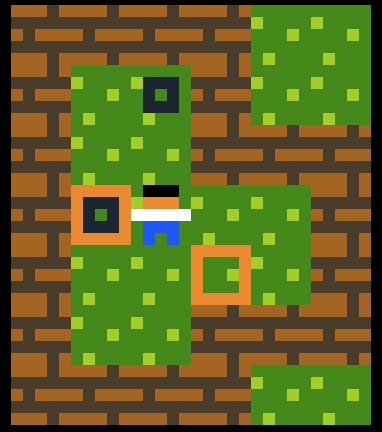
\includegraphics[width=0.40\textwidth]{images/sokoban.png}
    \caption{A simple PuzzleScript game}
    \label{fig:simple_game}
\end{figure}

PuzzleScript closely relates game design and game development through its Rule system. Many game mechanics in PuzzleScript games are literally defined with a single line. This makes it considerably easier to understand how alterations in the game code can affect game mechanics and gameplay. Such an example can be seen in Figure \ref{fig:push_mechanic} where a single line allows the player to push an entity in any direction. Reversing the arrow would allow the player to pull the entity, the entity can also be a reference to multiple entities allowing for a single line of code to affect multiple interactions. 

\begin{figure}
    \centering
    \begin{lstlisting}[language=PuzzleScript]
        [ $\color{violet}>$  Player | Crate ] $\color{BurntRed}->$ [  $\color{violet}>$  Player | $\color{violet}>$ Crate  ]
    \end{lstlisting}
    \caption{Code for push mechanics}
    \label{fig:push_mechanic}
\end{figure}

At its core, this rule system is a simple match and replace pattern. The designer defines a pattern on the left side that is either matched horizontally or vertically and then replaced with the pattern on the right side. In Figure \ref{fig:push_mechanic}, the patterns can be translated to "if a player tries to move into an adjacent crate, then move both entities in that direction". This simple core makes PuzzleScript very approachable by game designers of all levels and its flexibility still allows them to make relatively complex games. One of the contributions from the bachelor thesis by Vermeulen\cite{vermeulenautomated} is a prototype grammar to parse PuzzleScript. This provides support for generating code based on desired player affordances. The prototype parses a significant amount of PuzzleScript rules and serves as the foundation for our own grammar. As a prototype, it fulfills the role of parsing simple PuzzleScript games but it is not a complete grammar. Many of the finer details and corner cases of PuzzleScript's grammar are missing. We use the grammar and design formalization presented in the thesis as a stepping stone.

% Originally written in Dutch, a translator allowed us to make use of their work on reverse engineering PuzzleScript's grammar and of their prototype to get started.

% Several journals and personal accounts\cite{osborn2015playspecs}\cite{8901975}\cite{10.1145/2908812.2908920}\cite{6932896} help us understand PuzzleScript's popularity as a puzzle game engine and its appeal as a language for researching game design.

PuzzleScript's popularity as a game engine and its appeal as a case for researching game design is shown in several papers\cite{osborn2015playspecs}\cite{8901975}\cite{10.1145/2908812.2908920}\cite{6932896}. The papers provide a proof of PuzzleScript's popularity as a game engine with raw statistics and provide motivation arguments for its use within an automated game design perspective. The papers also discuss procedural content generation within PuzzleScript. The common thread between all these papers is that they demonstrate how the concepts we touch one can be used within PuzzleScript and how PuzzleScript is a legitimate case for realistic game research. In addition to Vermeulen's thesis, we also found other papers with interest in Procedural Content Generation. A paper by Krishnan\cite{krishnan2018level} is an example of people studying PuzzleScript games to research game design.

% During our research, we came across several prototypes that aimed to

Several projects that seek to extend or reimplement PuzzleScript in a different language already exist. They provided insights into the processes of the original JavaScript implementation and as such we felt it was important to give a brief overview. The PuzzleScript repository has 127 forks\footnote{\url{https://github.com/increpare/PuzzleScript/network/members}} at the time of writing, of those only a few are actively developed as extensions to PuzzleScript, the rest are either inactive or developed with the intent to merge back into the original with a pull request.

Pattern-Script\cite{PatternScript} is a major extension of the original PuzzleScript engine by Clement Sparrow. It aims to add a plethora of new features\footnote{\url{https://github.com/ClementSparrow/Pattern-Script/wiki}} and support for game designers. By providing additional keywords, the engine allows designers to use shortcuts for the creation of tilemaps and grants them a more granular control on the rule matching process. The extension does not modify the engine and does not extend the behavior of rules, instead it allows designers to restrict the conditions of the rules more tightly. This seems to go along our theory that extending PuzzleScript is hard because the engine's complexity.

This fork by Joe Osborn\cite{PuzzleScriptGA} claims to integrate game analysis but does not seem to have got any commits since the fork was made. Another example is the fork by Rikki Prince\cite{PuzzleScriptTracery} that attempts to make it possible to generate PuzzleScript games using grammar but does not provide working instructions. 

The implementations we found have similar goals to our own. However, unlike our approach, these implementations are all ports of the original PuzzleScript implementation with minor changes. We instead create a complete redesign of PuzzleScript that permits us to create algorithms and tools that can analyze its structure and semantic. This redesign is necessary for answering our research question and the reason we cannot use existing implementations for this project.

\begin{itemize}
    \item C\cite{puzzleengine}: Released, runs simple games.
    \item Rust\cite{puzzlescriptrust}: Released, feature-complete as far as we are aware, needs games to be formatted in a special JSON-based structure
    \item C++\cite{Psionic}: Released, missing features
\end{itemize}

Re-implementations provide insight into how other languages solve the technical complexity of PuzzleScript's rule system. The ones studied here all follow a similar approach to the original JavaScript implementation: hand-crafted parsers that statically check the game at the same time and tightly coupled phases.

Finally, we have works that extend the PuzzleScript implementation in small ways\cite{smoothscreen}\cite{irreversible}. These forks are usually created by programming-inclined PuzzleScript game designers, which have a specific need that the current implementation does not meet. The additions and modifications they perform provide insight into the needs of PuzzleScript developers and designers.

\section{Meta-programming}
Meta-programming is a programming technique that creates \emph{meta-programs}. Normal programs process and transform data, meta-programs process and transform other programs. Meta-programming techniques and language workbenches help programmers in the activities of meta-programming. Domain specific languages (DSL) are programming languages that perform a very specific set of tasks, compared to general-purpose languages which can be used for a wide range of tasks. PuzzleScript is an external DSL with the specific purpose of creating top-down or 2D puzzle games. One would be unable to use PuzzleScript to create websites or calculate financial data, that is outside the domain.

PuzzleScript makes use of meta-programming in its JavaScript implementation to transform rules into JavaScript functions. In this scenario, we see one of the limitations of this specific brand of meta-programming: code obfuscation. A significant part of the code that processes rules of a PuzzleScript game does not exist before runtime, this makes it much harder to maintain and extend. This decision hurts the readability and searchability of the codebase in that a programmer must first compile a game before being able to observe how the rules transform into code. Only having that complete overview during runtime makes it harder for programmers to identify and locate bugs.

Language workbenches can help to facilitate meta-programming. We use Rascal, a meta-programming language and language workbench to parse, run and analyze PuzzleScript games. We selected Rascal from a list of meta-programming languages and language workbenches identified by van Rozen\cite{10.1145/3412843} and in a paper on language workbenches for game development\cite{10.1007/978-3-319-02654-1_3}. Domain-specific languages have been successfully applied in many domains but their benefits to game development are not yet clear. According to this paper by Klint and van Rozen\cite{10.1007/978-3-319-02654-1_3}, this is due to the game domain being very diffuse. It is hard to analyze a moving domain where modeling and software reused are limited. The existing approach is game engines which provide the ability for software reuse and optimization, but even these have very specific cases and no silver bullet exists.

In this thesis on the state of the art in workbenches, several other language workbenches are identified. It also identifies several features deemed essential in language workbenches and compares the identified list with the workbenches themselves. From that, we can see Rascal is not the most feature-complete of the workbenches presented, but it provides the ability to make up that difference programmatically. 

Rascal is an extensible meta-programming language and IDE for source code analysis and transformation with the goal to merge the SCAM (source code analysis and manipulation) domain into a single language\cite{Klint2011}. It provides parsing in the form of its Syntax Definition Formalism that allows developers to create a literal representation of the programs they are trying to parse through the use of lexical and symbols. These representations can then be converted by \textit{imploding} them into equivalent data structures. Rascal also offers the possibility of processing concrete syntax which does not require implosion but has other downsides. Rascal also implements the concept of \textit{visiting}, which allows us to traverse an arbitrarily complex subject and apply a number of cases to all its nodes. We can use this to enrich a parse tree without having to modify its structure by editing or replacing individual nodes.


Finally, Rascal presents a concept called "Abstract Patterns" which allows us to match data structures using regular patterns similar to how one might match text with regular expressions. This concept is very similar to the way that PuzzleScript Rules work on the surface and as such we believe that it is possible to use it to create a more human-readable version of compiled Rules. In the current implementation, Rules are compiled into functions, which adds a layer of complexity as part of the codebase that can only be observed during runtime.  

\section{Reverse Engineering}
Our project aims to create a version of PuzzleScript that is well suited for game design research, extension and maintainability. Unfortunately, we cannot simply port the existing JavaScript implementation. We need access to PuzzleScript's design to create our own implementation. Since the design of PuzzleScript is not fully documented, we have to reverse engineer the existing implementation.

Reverse engineering is the method of attempting to understand how a program works by deductive guesses based on the observation of the program's behaviors\cite{10.1145/336512.336526}. Researchers who reverse engineer programs do not always have access to the full source code or architecture documents and as such must rely on their observations to guess the original intentions of the developers. There are two main aspects to reverse engineering: redocumentation and design recovery. Redocumentation is the process of creating a new representation of a program and design recovery is the process of using deduction in relation to one's experience with the product to recover its design\cite{43044}.

Reverse engineering is commonly used in cases where the source code is inaccessible, however, that is not a requirement. Reverse engineering can also be used when the source code is not properly documented or densely structured to reconstruct the design of the application. This method is not without flaws, it requires a good understanding of the language the program is written in. Knowledge gaps can sometimes be filled by observing the behavior of the application from the user perspective. Reverse engineering is very time consuming, but it is sometimes the only option to be able to separate the design from the implementation.

The process of design recovery involves connecting the codebase to user-facing endpoints to understand how they fit together. Observing the behavior of a program is a relatively safe way of ensuring that the correct intent is understood, but it depends heavily on managing to trigger every corner case. Complementing this is the method of going through the codebase\cite{10.5555/2555229}. This method presents its own set of issues depending on how strict the language is with its typing. 

The end product of design recovery is a design document based on the observed behaviors. This document is made up of assumptions the person conducting the reverse engineering made therefore it is not a pure version of the original design. Purifying that version to be closer to the original is a task that requires a lot of work but can be supported by specialized techniques such as model-based reverse engineering\cite{DBLP:journals/computer/Biggerstaff89}.


\chapter{Reverse Engineering PuzzleScript}
\label{ch:puzzlescript}
In this chapter, we take steps to extract PuzzleScript's design from its implementation through reverse-engineering the JavaScript implementation. As we previously mentioned, the reason we need to reverse engineer PuzzleScript is that the existing implementations are not suitable for our research purposes. Therefore, we create our own. However, PuzzleScript does not have a complete design document we can use\footnote{\url{https://groups.google.com/g/puzzlescript/c/UBe9M8QP-rk}}. We need a design document because we do not want our implementation to have similar pitfalls as the official implementation.

% However, to create our own, rather than porting an existing implementation, we need to be able to implement the design but PuzzleScript does not have a complete design document. 

% The design document resulting from this step is one of the contributions of this project.

\section{Approach}
We create a comprehensive PuzzleScript design document by performing design recovery on the existing implementation by Lavelle. Design recovery in our case involves going through the codebase and observing the behavior of the implementation. We have access to the codebase through the public GitHub repository and we can access the deployed implementation on the PuzzleScript website\footnote{\url{https://www.puzzlescript.net/editor.html}}.

Investigating PuzzleScript's codebase presents challenges. JavaScript is dynamically typed, which means that the type of variables and function returns is not guaranteed. For instance, the code \texttt{a + b} could be adding two integers together or concatenating two strings. The only way of guaranteeing either outcome is to run the code and observe it. We can use context clues such as comments and variable names in the early stages but validation requires the code to be observed during runtime. Comments are sparse in PuzzleScript's codebase and the code density is high. As a result, reverse engineering the design of the codebase is challenging. Recovering the design also relies on the software engineer knowledge of that specific language. We complement our approach by observing the program during runtime. We do this by subjecting the system under study to various inputs to observe its behavior. We combine both approaches to create the design document.

Part of PuzzleScript's design is documented in the bachelor thesis by Vermuelen\cite{vermeulenautomated}. Their thesis breaks down the design of PuzzleScript and implements that design using Rascal's Syntax Definition. This is similar to our approach, however, their design document and implementation are incomplete. Their goal is to generate code from keywords and their implementation serves that purpose. Our goal is to parse every PuzzleScript game in existence using a new  grammar that can be reused in future prototypes. As such, we need a design document that is more comprehensive and documents PuzzleScript's many corner cases.


\section{PuzzleScript's Design}
In this section, we describe the results of our reverse engineering. We frequently reference the PuzzleScript user manual\footnote{\url{https://www.puzzlescript.net/Documentation/prelude.html}}. The user documentation focuses on the specifics of games. We instead focus on the general syntax structure of PuzzleScript and on the contextual constraint that can be used for creating a static analyzer. We aim to provide a document that makes it easier to parse PuzzleScript while the user guide provides specific implementation details.

\subsection{General}
A PuzzleScript file stores the contents of exactly one \emph{game}. Anything within that file is considered content for that game and that game only. There exists no way of splitting a game into multiple files or storing more than one game into a single file.

A \emph{game} consists of a \emph{prelude} and multiple \emph{sections}. Sections consist of a header which is the name of the section between two optional lines of equal (=) sign. Sections are delimited by either two headers or a header and the end of the file. In the JavaScript implementation, these sections must be in a specific order but from a design perspective, there is no inherent need for a specific order. However, "define before use" is a natural policy of programming and PuzzleScript may rely on that. The grammar of a section's content depends on the section itself. PuzzleScript is a context-sensitive grammar. The rules of syntax apply differently based on the context, in this case the context is the section. The order of the sections is as follows:
\begin{itemize}
    \item Objects: Defines all objects to be used in the game
    \item Legend: Create shorthand links between symbols and objects to allow properties, aggregation of objects, and tilemap creation.
    \item Sounds: Defines handlers to play sounds when certain events happen
    \item Layers: How objects interact with each other movement-wise, whether they can stack or if they collide
    \item Rules: How objects interact, what happens when certain items are next to each other or if a player tries to move into a certain item
    \item WinConditions: Defines victory conditions for the level
    \item Levels: List of tilemaps and messages that represent the different rooms the player will explore
\end{itemize}

\emph{Comments} in PuzzleScript are delimited by parenthesis (\emph{()}) and can be placed anywhere. It is unclear whether that is a conscious decision or simply a byproduct of the fact that the engine strips all comments before compiling the game.

\subsection{Prelude}
A game's \emph{Prelude} consists of all the lines before the first section. Each line consists of one or two tokens: a \emph{keyword} and a \emph{value}. These pairs allow the developer to modify how the engine works and the visual aspect of the game. Certain keywords do not require a value, they simply need to appear in the prelude to have an effect. Values can be a string (a list of tokens displayed literally), a numeral (int or float), or a member from an enumerator. A full list of possible prelude keywords and their values is documented in PuzzleScript's user guide\footnote{\url{https://www.puzzlescript.net/Documentation/prelude.html}}. 

\subsection{Objects}
\emph{Object} are the building blocks of PuzzleScript's games. They make up everything the player can see and interact with. They are used in rules to define game mechanics, they are used in conditions to define how the player achieves victory and they are used in levels to define what kind of challenges they present.

An object consists of a \emph{name}, an optional \emph{legend}, a list of \emph{colors} and an optional \emph{sprite}. The name and the legend are on the same line, the color list on its own line, and the sprite is a 5x5 tilemap. Colors are either an HTML color code or a color keyword from the selected palette. The color palette available is decided by the developer in the prelude from a wide range. The sprite is a 5x5 tilemap of where the \texttt{.} represent a transparent pixel and numbers from \texttt{0-9} represent a colored pixel based on the index of the colored list. As can be seen in Figure \ref{fig:object_code}, \texttt{0} represents blue because it is the first color in the list of colors defined for that object.

\begin{figure}
    \centering
    \begin{lstlisting}[language=PuzzleScript, xleftmargin=2pt, , basicstyle=\ttfamily\footnotesize]
        Player
        black $\color{BurntOrange}orange$ $\color{darkgray}white$ $\color{blue}blue$
        $\color{black}.000.$
        $\color{black}.$$\color{BurntOrange}111$$\color{black}.$
        $\color{darkgray}22222$
        $\color{black}.$$\color{blue}333$$\color{black}.$
        $\color{black}.$$\color{blue}3$$\color{black}.$$\color{blue}3$$\color{black}.$
    \end{lstlisting}
    \caption{An object}
    \label{fig:object_code}
\end{figure}

The name and legend of the object can be almost any character, although choosing certain characters can be an issue in other sections. For example, naming an object using any of the directional arrows is technically allowed. However, that makes it impossible to use the object's name in a rule, where the directional arrows are reserved keywords. In other cases, using reserved keywords for objects still works but confuses the syntax highlighter and results in code that is difficult to read and understand to the programmer.

\subsection{Legend}
\emph{Legend} allow the developer to create shorthand references to one or more objects. A legend consists of a name and a sequence of references, separated by the equal (=) sign. The sequence of object references, either the object name or another legend, is separated by either 'and' or 'or'. Legend cannot mix separators and cannot reference a legend that makes use of the other separator. \emph{Properties} are object references separated by 'or'. Properties are used to reference multiple objects in the context of rules, victory conditions, and sound. \emph{Aggregates} are object references separated by 'and'. Aggregates represent objects that are stacked on top of each other. Aggregates are used to place multiple items on one pixel in Level tilemaps.

The name of the legend is subject to the same constraints as the name of an object. Aggregates and legends referencing a single object can be used on tilemaps as long as the legend name is only one character long. An example of the different combinations can be seen in Figure \ref{fig:legend_code}.

\begin{figure}
    \centering
    \begin{lstlisting}[language=PuzzleScript]
        Obstacle = Crate $\color{violet}or$ Wall
        P = Player
        O = Target $\color{violet}And$ Crate
    \end{lstlisting}
    \caption{Three legends}
    \label{fig:legend_code}
\end{figure}

\subsection{Sound}
\emph{Sounds} allow the game designer to define what sound to play in the case certain events happen. A sound consists of either a reference or a sound keyword (SFX[0-10]) followed by a list of conditions (moving left, stationary) and finally a sound seed. The editor generates a limited range of sound seeds for use within games. Examples of sounds are shown in Figure \ref{fig:sound_code} and the possible conditions are documented in PuzzleScript's user documentation\footnote{\url{https://www.puzzlescript.net/Documentation/sounds.html}}.

\begin{figure}
    \centering
    \begin{lstlisting}[language=PuzzleScript]
        player $\color{violet}move  up$ $\color{BurntOrange}142315$
        Player $\color{violet}Move  down$ $\color{BurntOrange}142313$
        Player $\color{violet}Move  right$ $\color{BurntOrange}142311$
        Crate $\color{violet}Move$ $\color{BurntOrange}412312$
        Player $\color{violet}CantMove up$ $\color{BurntOrange}41234$
        Crate $\color{violet}CantMove$ $\color{BurntOrange}41234$
        Crate $\color{violet}Create$ $\color{BurntOrange}41234123$
        $\color{violet}CloseMessage$ $\color{BurntOrange}1241234$
        Sfx0 $\color{BurntOrange}213424$
        Sfx3 $\color{BurntOrange}213424$
    \end{lstlisting}
    \caption{Combinations of keywords creating sound events}
    \label{fig:sound_code}
\end{figure}

\subsection{Collision Layers}
Layers are lines of sequences that consist of either object reference or properties separated by either an optional command (,) or a white space. The purpose of the section is to define whether objects can stack or if they collide. All objects defined in the game must be referenced in a layer. This restriction exists so that the developer does not accidentally spawn an object without collision. Referencing an object in multiple layers is technically allowed but not recommended and it raises a warning. Ignoring the warning can have unintended consequences such as layers being ignored, allowing for unintended movement. Figure \ref{fig:layer_code} illustrates an example of a layer.

% An example of a layer can be seen in Figure \ref{fig:layer_code}.

\begin{figure}
    \centering
    \begin{lstlisting}[language=PuzzleScript]
        Crate, Player, Wall
    \end{lstlisting}
    \caption{A Layer}
    \label{fig:layer_code}
\end{figure}

\subsection{Rules}
Rules are at the heart of PuzzleScript. A rule consists of a series of prefixes that affect the whole rule, a left-hand side \emph{"pattern"} and a right-hand side \emph{"replacement"}. 

The left-hand side must contain at least one \emph{rule part}, the right-hand side must contain 0 or exactly the same number of rule parts as the left-hand side.  Rule parts start with a \texttt{[} and end with a \texttt{]}. Within a rule part, there are a certain number of \emph{rule sections}, each rule part on the right must have the same number of sections as the equivalent rule part on the left. Sections of a rule part are separated by \texttt{|}. Each section consists of object references that can stack, and each object can have one \emph{modifier}. Modifiers allow checking for special matches such as moving objects or the absence of an object. Each section represents an adjacent cell, either vertical or horizontal. Rules can be marked as "late" which means they will run in a second phase after the player movement has been processed. More information on the rules and the modifiers can be found in PuzzleScript's user manual\footnote{\url{https://www.puzzlescript.net/Documentation/rules.html}}. Figure \ref{fig:rule_code} illustrates a few examples of Rules.

\begin{figure}
    \centering
    \begin{lstlisting}[language=PuzzleScript]
        [ $\color{violet}>$  Player | Crate ] $\color{BurntRed}->$ [  $\color{violet}>$  Player | $\color{violet}>$ Crate  ]
        $\color{violet}late$ [ Crate | Crate | Crate ] $\color{BurntRed}->$ [ | |]
    \end{lstlisting}
    \caption{A few Rules}
    \label{fig:rule_code}
\end{figure}

\subsection{Win Conditions}
\emph{WinCoditions} offer a simple way of creating victory conditions that determine when a player has completed  (or won) a level. If no conditions are defined, the player will be unable to win a level. If multiple conditions are defined then all of them must be true simultaneously for the player to win. A condition consists of a victory keyword, an object reference or a property, and an optional 'on' condition. An 'on' condition consists of the word 'on' and an object reference. Conditions check whether an object exists on the level (or does not exist). The 'on' condition further requires that the object referenced in the condition be on the same XY-coordinates as the object referenced in the 'on' condition.

Valid keywords for a condition are \texttt{Some}, \texttt{No} and \texttt{All}. A condition with the \texttt{Some} keyword becomes true if at least one of the objects referenced is present on the level. If the 'on' condition is defined, it becomes true if at least one of either object is stacked on the other. A condition with the \texttt{No} keyword becomes true if zero objects are present on the level. If the 'on' condition is defined, then it becomes true if zero of either object are stacked. A condition with the \texttt{All} keyword cannot be used without the 'on' condition being defined. With the 'on' condition defined it becomes true if all objects referenced in the 'on' condition are stacked with an object from the condition. A few examples of these conditions can be seen in Figure \ref{fig:conditions_code}

\begin{figure}
    \centering
    \begin{lstlisting}[language=PuzzleScript]
        $\color{violet}Some$ target $\color{violet}on$ crate
        $\color{violet}No$ Player
        $\color{violet}All$ oranges $\color{violet}on$ plates
    \end{lstlisting}
    \caption{Three win conditions}
    \label{fig:conditions_code}
\end{figure}

We note that the syntax of the "Object1 on Object2" syntax can be confusing, and perhaps even misleading. For example, in the case of \texttt{All Crate on Target} what this means is that there cannot be a target that is not on the same XY coordinate\footnote{We define "stacked" as being on the same XY coordinate as PuzzleScript does not require for a specific item to be on top, as such, an item can still be on another item even if that first item is actually under.} as a Crate. However, from a natural language point of view, one would assume the contrary, that each Crate must be on the same XY as a Target. This distinction is important when there is more of Object1 than of Object2. For example, if there are four Target and three Crate then the level is impossible to win.

\subsection{Levels}
The level section consists of a combination of any number of \emph{Levels} and \emph{Messages}.  A Level is a rectangular 2-D tilemap of variable width and height that consists of symbols representing one or more objects. Only one character long reference can be used, whether they are legend or object names. Aggregation can also be used in levels but not properties.

A Message is a single line consisting of the word 'message' followed by a string (multiple words). When the Level before the message is completed, the engine will display the message before moving on to the next level. Any number of messages can be defined in between two levels, before the first level or after the last level. An example of a Message and Level can be seen in Figure \ref{fig:level_code}.

\begin{figure}
    \centering
    \begin{lstlisting}[language=PuzzleScript]
        $\color{violet}message$ $\color{BurntOrange}Level 1: Beginnings$
    
        ####..
        #.O#..
        #..###
        #@P..#
        #..*.#
        #..###
        ####..
    \end{lstlisting}
    \caption{A message and a level}
    \label{fig:level_code}
\end{figure}

\section{Implementation of PuzzleScript}
Here we describe the design decision of the 'official' implementation of PuzzleScript written by the original developer, Stephen Lavelle, in JavaScript.

The JavaScript implementation of the PuzzleScript engine consists of three separate phases. First, the source code is \emph{parsed} and checked for validity. Second, the \emph{compiler} transforms the parsed code into JavaScript data structures. This also involved transforming rules into JavaScript functions using meta-programming. Further verification is conducted during compilation. Finally, the \emph{engine} runs the game and awaits player input.

The repository containing the source code for PuzzleScript consists of 27 files and adds up to over 15,000 lines of code calculated using \emph{cloc}\footnote{\url{http://cloc.sourceforge.net/}}. Most of the files are used to store code that provides features not directly tied to PuzzleScript's design such as Saving/Exporting games. Those files also contain code for features that are small parts of the design but require large implementations such as sounds. Three files are responsible for the phases we identified above and total 5820 lines of code. The files are: \begin{itemize}
    \item parser.js: 1065 lines, responsible for the Parsing phase.
    \item compiler.js: 2350 lines, responsible for the Compilation phase.
    \item engine.js: 2405 lines, responsible for the Engine phase.
\end{itemize}

The in-browser IDE, a vital part of the implementation, is implemented using CodeMirror. CodeMirror is a versatile library specifically made for editing code in-browser. The IDE provides comprehensive syntax coloring that adapts to its context. Pixels representing a color will appear as that color in the respective sprites that use them. Syntax coloring will fail if the syntax is incorrect. 

\begin{figure}[h]
    \centering
    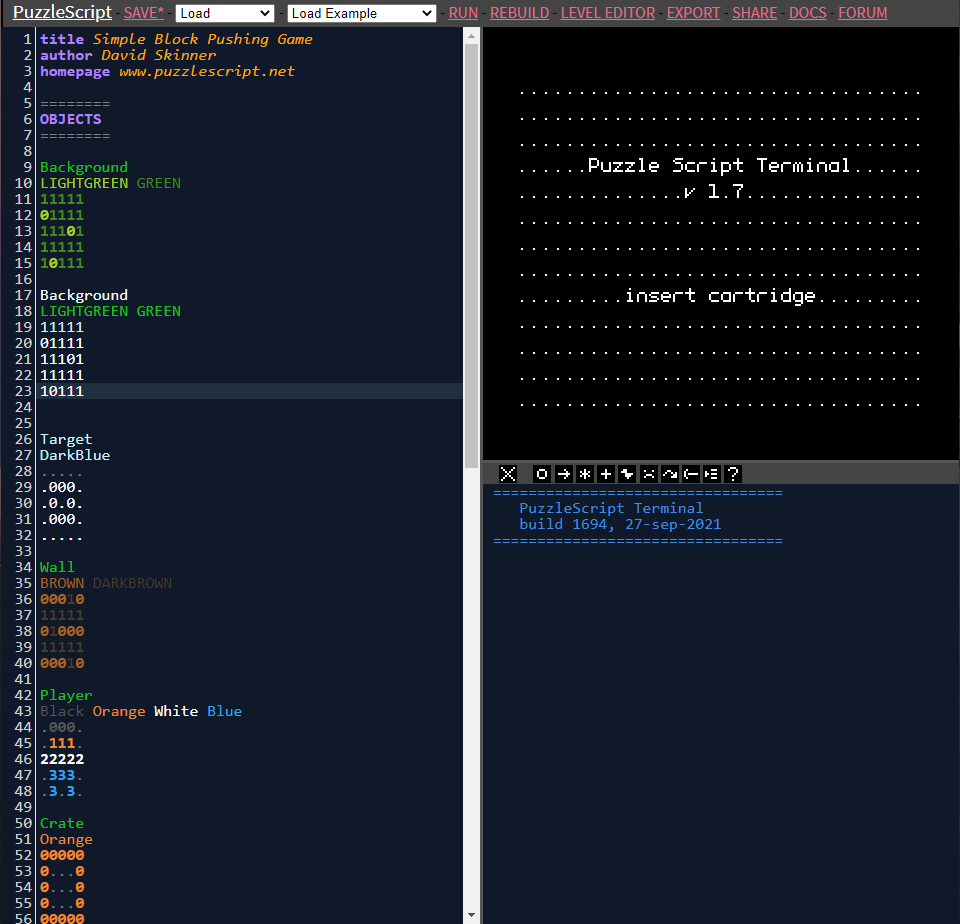
\includegraphics[width=1\textwidth]{images/PuzzleScript_IDE.png}
    \caption{PuzzleScript's browser IDE}
    \label{fig:browser_ide}
\end{figure}

Once the user presses "Run" the game compiles, errors appear in the bottom right and the title screen for the game appears in the top right. The top bar of the IDE provides additional options for sharing and exporting the game into a standalone application alongside helpful links for seeking support.

The implementation displays error messages as they are detected and aborts the compilation if a certain threshold is reached. The threshold is necessary because of the possibility of an error cascade. Without the threshold, a high number of ghost errors might be displayed. This would make it harder to fix the true issues. With the threshold, the developer is encouraged to address errors one by one, allowing the static checker to clear up any ghost errors. User inputs are context-sensitive. If the user presses an arrow key while focused on the editor, it will move their cursor text, if they do the same with a focus on the game, it will attempt to move their character. The IDE does not have a contextual right-click menu.

\section{Lessons Learned}
Here we analyze and discuss design decisions that complicate Puzzlescript's analysis. In particular, we discuss how language features lead to possibly complex situations when writing Puzzlescript due to 'dark corners' in the language semantics.

\subsection{Compilation}
PuzzleScript is an incredibly flexible language, both in design and through implementation. However, this flexibility includes corner cases in language semantics that make it hard to formalize the semantics.

For instance, PuzzleScript has section-specific reserved keywords. For instance, specifying the legend for an object as \textbf{]} is allowed. However, the trade-off is that the legend cannot be used to reference that object in the Rules section since \textbf{]} is a reserved keyword in the context of that section. This is made possible by the technical implementation of PuzzleScript's parse which is line-based and handcrafted. The flexibility of PuzzleScript's grammar places it in the category of context-sensitive grammars. Section-specific keywords are not a common design pattern. PuzzleScript's grammar leveraging that pattern poses a challenge to formalizing it.

% places PuzzleScript's grammar in the category of context-sensitive grammars.

% The question we pose now is whether or not this flexibility is worth the extra complexity. The flexibility makes it hard to create a formal grammar because section-specific keywords are not a common design pattern. 

The JavaScript implementation has tightly coupled compiler phases. This means that extending the codebase requires a full understanding of the entire process. There are no "general" functions that can be simply provided as a set of instructions for extensions. PuzzleScript does not provide an interface with helper functions but rather defines functions based on the current needs of the implementation.

\subsection{Intentional Ambiguities}
The design of PuzzleScript includes intentional ambiguities. Components can be defined in multiple ways with slight differences to their syntax. These multiple ways do not affect the behavior of the component but need to be handled by the parser. These variants of the syntax provide no real benefit and may even confuse the game designers. For instance, objects in collision layers are normally separated by a comma, making the formalization of the grammar appear simple. However, upon further inspection, we discover that a list of space-separated objects is also a valid line. This means that there are three possible separators for a collision layer that can be used interchangeable: 1) a comma with no whitespace; 2) a comma and a white space (in any order) and 3) just a whitespace.

% This means that the comma is no longer a separator but rather an optional token that may or may not separate objects. Three valid examples of the same layer can be seen in Figure \ref{fig:Layer Example}.

\begin{figure}[!t]
\begin{lstlisting}[language=PuzzleScript]
Crate,Player, Target
Crate Player Target
Crate, Player Target
\end{lstlisting}
\vspace*{-8pt}
\caption{Three examples of the same layer}
\label{fig:Layer Example}
\vspace*{-8pt}
\end{figure}

\subsection{Rule Semantics}
Rules, the heart of PuzzleScript, are complex to read and hard to maintain. The instructions of the rules are transformed into code which the compiler interprets as a JavaScript function. PuzzleScript's engine makes use of meta-programming as it generates the JavaScript code that represents the rules during runtime as a function. This means that a great part of the engine does not exist until runtime. Because JavaScript is dynamically typed, it is hard to understand what is being passed to these functions. 

In the JavaScript implementation, parsing is one of the two phases and is done simultaneously with error checking. This can very easily cause errors to cascade since any error also throws the parser off as can be seen in Figure \ref{fig:error_cascade}. The graphics and engine are similarly coupled, graphics are generated as rules are applied, and the objects have methods for generating graphics directly attached to them. Additionally, the error messages are duplicated throughout the process. This means that if a developer wants to change the wording of an error message, they need to go through the core files and modify every instance of the message.

\begin{figure}[!t]
    \centering
    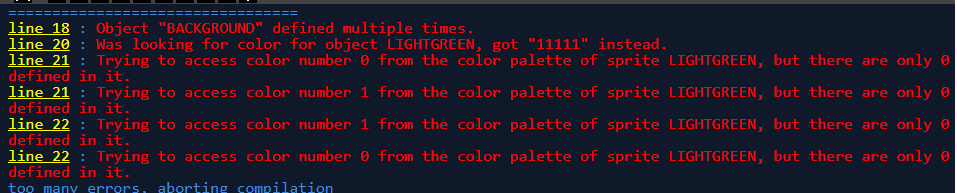
\includegraphics[width=1\textwidth]{images/Example_errors_current.png}
    \caption{A single error causes a cascade of ghost errors}
    \label{fig:error_cascade}
\end{figure}

\subsection{Interactive Development Environment}
The IDE itself is simple, offering syntax coloring, and printing errors. Its real power comes from the engine itself, which allows running games with great performance directly in the browser. When an error occurs, the syntax coloring breaks on the line where the error occurred. This allows for basic debugging but does not provide any information on what the error is. The debug console provides the necessary information to solve most errors. However, it usually only provides enough information to solve the first error encountered. Both of these aspects are functional and serve their purposes but have room for improvement.

\section{Conclusion}
We conclude that PuzzleScript is a complex language that appears simple to the users. The implementation focuses on performance and portability at the cost of extensibility and maintainability. This specific focus makes it hard to use to answer our research questions, as such, we design our own implementation.

\chapter{ScriptButler}
\label{ch:research}
Here we present ScriptButler, a prototype tool for analyzing PuzzleScript games. The tool aims to give game designers a better understanding of how code changes affect gameplay. As previously mentioned, we created this prototype because the official PuzzleScript implementation is unsuitable for our research goals. Therefore, to resolve this issue we create our own design and implementation of PuzzleScript. We base our implementation on the design document we reverse engineered in the previous chapter. In this chapter, we discuss the design decisions we take. Our aim with this implementation is to create a general-purpose tool capable of parsing, validating, and running games. Additionally, for the purpose of this project, we also design a dynamic analysis module to provide support for analyzing gameplay. The dynamic analysis module also demonstrates the extensibility of our prototype.

Figure \ref{fig:scriptbutler_flow} shows an overview of our tool's architecture. The game designer interact with the tool through the IDE and the Web GUI. These two components provide user-friendly endpoints to our tool and are responsible for sending inputs from the game designer to the tool. ScriptButler is split up into multiple phases, this is done to reduce issues tied to coupling. The parser is our grammar, it reads PuzzleScript code and converts it into Rascal data structures. The post-process phase cleans up those data structures and annotates them to provide an outline and syntax coloring. The static checker verifies the validity of the code and provides error messages that the IDE can display to the game designer. The compiler further transforms the data structures, removing unnecessary content and making them more efficient to run in our engine. The engine run the game and displays the result in the Web GUI. The user can send inputs to the engine using that GUI and get debugging information. Finally, the dynamic analyzer runs tests on the compiled version of the game and provides feedback on the gameplay as messages that the IDE can display. We explain all the sections in greater detail in the following sections. 

\begin{figure}[!t]
    \centering
    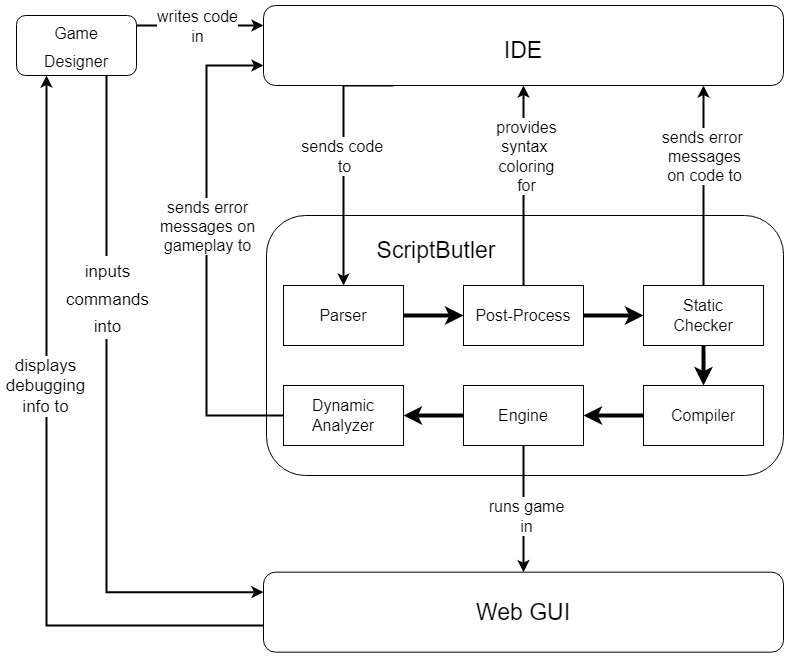
\includegraphics[width=1\textwidth]{images/ScriptButler Flow.png}
    \caption{The data flow through ScriptButler and its extensions}
    \label{fig:scriptbutler_flow}
\end{figure}

\section{Redesigning PuzzleScript with Rascal}
\newcommand{\dd}{\textsuperscript{[D]}}
Here we present the design of the PuzzleScript implementation we created using the design document we obtained by reverse-engineering the JavaScript implementation. Design decisions that arise from that understanding and that differ from the design decisions of the original implementation are marked with "\dd". When designing the implementation, we use a test-driven approach. We write the tests and their expected results based on the reverse engineering of the original implementation. We then implement PuzzleScript's design and frequently test our implementation against the tests. One of the goals for our implementation is to be compatible with existing games and the tests ensure we keep in line with that goal.

Our second goal is to create a design that is more maintainable than the original JavaScript one. Rascal satisfies part of that goal as a statically typed language. This makes it easier for programmers to understand the data flow. We also leverage good engineering practices such as self-documentation through the use of relevant variables and function names. Our third and final goal is creating an extensible design. To achieve this, we design our implementation with loose coupling between modules. Instead of creating a monolithic structure, we create a collection of plugins that are handled by a general function in charge of passing the data from one plugin to the other. Our approach makes it easy to add, remove or modify plugins. In the rest of this chapter, these plugins are called phases as they mirror, to an extent, the phases of compilation.

We split up the design of our implementation into separate phases\dd. Each phase has progressively stricter requirements on what counts as valid code. The phases are the following:
\begin{itemize}
    \item Parsing: Using a flexible formalized grammar, a PuzzleScript file is read and transformed into a parsed tree
    \item Post-process: The parsed tree is cleaned up and enriched with meta-data
    \item Static Check: Components of the file are checked for validity according to the specifications extracted from the JavaScript implementation.
    \item Compilation: The game is compiled into a form the engine can run, converting the AST to more efficient Rascal data structures
    % \item Dynamic Check: By running sections of the game using the engine, additional messages are generated on the gameplay
    \item Run: The game is running, allowing for the player to interact with it
    % \item Post-game analysis: Stats collected during the running phase are displayed
\end{itemize}

Splitting the compilation process into separate phases enables us to parse invalid code without the process aborting at the first error. The behavior assists designers in identifying multiple issues simultaneously.  We also separate the backend (parsing, checking, compiling) from the frontend (editor, interface)\dd. The backend is designed to accept source code, generate the data structures, and alter those data structures based on user input. The front end acts as a wrapper around the backend, communicating through specific endpoints. The approach allows us to decouple the user interface and engine, making it easier to alter either without impacting the other. Developers can even create their own implementation of the frontend or backend with seamless integration.

The design document of PuzzleScript is subject to errors of misinterpretation because it is based on reverse engineering. We mitigate these interpretation issues by verifying the design of our implementation against the behaviors of the official implementation. We go further into our verification process in Section \ref{sec:testing}.

\subsection{Parsing}
We address the need for a reusable and maintainable parser by creating a formal syntax definition in the form of a grammar. In our design, we make several important changes to this phase. However, we want our redesign to remain compatible with the PuzzleScript design. As such, it is important that this phase's user-facing endpoints do not change. The main design change in this phase is that we switch from using a hand-crafted parser to using Rascal's Syntax Definition feature\footnote{\url{https://docs.rascal-mpl.org/stable/RascalConcepts/\#RascalConcepts-SyntaxDefinitionAndParsing}}\dd. This decision allows us to create a declarative representation of a PuzzleScript file that consists of lexicals and symbols. This representation is human-readable and easier to extend than a line-based parser. 

A Rascal syntax definition consists of a layout, keywords, lexicals, and symbols. The layout is a pattern that matches the white space and comments, it can be seen at the top of Figure \ref{fig:PuzzleScript Lexicals}. Symbols are composed of lexicals, literals, and other symbols. We use lexicals to parse individual tokens and then group them into symbols that represent PuzzleScript components such as Objects, Rules, Sprites and many more. Figure \ref{fig:syntax_example} shows a simple example using practically all Syntax Definition features.

\begin{figure}[!t]
\begin{lstlisting}[language=rascal]    
// layout is lists of whitespace characters
layout MyLayout = [\t\n\ \r\f]*;

// identifiers are characters of lowercase alphabet letters, 
// not immediately preceded or followed by those (longest match)
// and not any of the reserved keywords
lexical Identifier = [a-z] !<< [a-z]+ !>> [a-z] \ MyKeywords;

// this defines the reserved keywords used in the definition of Identifier
keyword MyKeywords = "if" | "then" | "else" | "fi";

// here is a recursive definition of expressions 
// using priority and associativity groups.
syntax Expression 
  = id: Identifier id
  | null: "null"
  | left multi: Expression l "*" Expression r
  > left ( add: Expression l "+" Expression r
         | sub: Expression l "-" Expression r
         )
  | bracket "(" Expression ")"
  ;
\end{lstlisting}
\vspace*{-8pt}
\caption{Syntax example}
\label{fig:syntax_example}
\end{figure}

The main weakness of using Syntax Definition is that we lose control over how the parser handles invalid code. If the parser runs into invalid code it raises an error intended for the tool designer. This error is hard to read for the tool user and does not provide the necessary feedback for a game designer to fix their code. To address this issue, we create a \emph{'flexibile'} grammar. This means that our grammar should parse and accept invalid code, to an extent. We aim to design our grammar so that only severe structural errors can cause it to raise an error. To this end, we define keywords to make our definition more human-readable. However, we do not use them to exclude tokens to avoid a parser error. Our grammar is mostly made up of flexible lexicals grouped up under symbols. The main goal of our grammar is to assign "labels" to tokens so that our static checker knows what rules they should be checked against. Figure \ref{fig:PuzzleScript Lexicals} shows the lexicals, and Figure \ref{fig:example_symbol} shows a sample of our grammar that parses Objects. The latest version of the full grammar can be accessed on the project repository\footnote{\url{https://github.com/ClementJ18/ScriptButler/blob/main/src/PuzzleScript/Syntax.rsc}}.

The Syntax Definition also offers an opportunity to annotate the file with interesting metadata. This metadata can then be used by the syntax checker or IDE plugins to enrich and support the developer experience. For example, the \texttt{@Foldable} tag, allows the developer to collapse any piece of code that matches the symbol in the IDE to temporarily hide it. The design of our grammar does still present weaknesses. PuzzleScript's design presents several ambiguities which a formal grammar cannot handle. We mitigate the effect of these ambiguities by defining certain objects more rigidly. This approach directly counteracts our goal of keeping the grammar flexible so we carefully balance the two. 

The result of this section is a grammar that we can apply directly to a PuzzleScript file to generate a parse tree representing that game. The parse tree needs further manipulation to be usable but using a Syntax Definition fulfills our goal of creating a more readable version of PuzzleScript's grammar.

\begin{figure}[!t]
\begin{lstlisting}[language=rascal]
lexical LAYOUT 
	= [\t\r\ ]
	| ^ Comment Newlines
	> Comment
	;
layout LAYOUTLIST = LAYOUT* !>> [\t\r\ )];

lexical SectionDelimiter = [=]+ Newlines;
lexical Newlines = Newline+ !>> [\n];
lexical Comment = @Category="Comment" "(" (![()]|Comment)+ ")";
lexical Newline = [\n];
lexical ID = @Category="ID" [a-z0-9.A-Z#_+]+ !>> [a-z0-9.A-Z#_+] \ Keywords;
lexical Pixel = [TRUNCATED];
lexical LegendKey = Pixel+ !>> [TRUNCATED] \ Keywords;
lexical Spriteline = [0-9.]+ !>> [0-9.] \ Keywords;
lexical Levelline = Pixel+ !>> Pixel \ Keywords;
lexical String = ![\n]+ >> [\n];
lexical SoundIndex = [0-9]|'10' !>> [0-9]|'10';
lexical KeywordID = @Category="Key"[a-z0-9.A-Z_]+ !>> [a-z0-9.A-Z_] \ 'message';
lexical IDOrDirectional = @Category="ID" [\>\<^va-z0-9.A-Z#_+]+ !>> [\>\<^va-z0-9.A-Z#_+] \ Keywords;
\end{lstlisting}
\vspace*{-8pt}
\caption{PuzzleScript layout and lexicals}
\label{fig:PuzzleScript Lexicals}
\end{figure}

\begin{figure}[!t]
\begin{lstlisting}[language=rascal]    
syntax Objects = objects: SectionDelimiter? 'OBJECTS' Newlines SectionDelimiter? ObjectData+;
syntax Color = @category="Color" ID;
syntax Colors = Color+;
syntax ObjectName = @category="ObjectName" ID;

syntax ObjectData
	= @Foldable object_data: ObjectName LegendKey? Newline Colors Newline Sprite?
	| object_empty: Newlines
	;
	
syntax SpritePixel = @category="SpritePixel" SpriteP;

syntax Sprite 
    =  @Foldable sprite: 
       SpritePixel+ Newline
       SpritePixel+ Newline
       SpritePixel+ Newline 
       SpritePixel+ Newline
       SpritePixel+ Newline
    ;
\end{lstlisting}
\vspace*{-8pt}
\caption{Symbols for parsing Objects}
\label{fig:example_symbol}
\end{figure}

\subsection{Post Processing}
% not sure what else to explain without getting technical // TODO: Ask Riemer
The post-processing phase aims to make it easier to manipulate game code programmatically and pad the weaknesses of the grammar. During this phase, we annotate the parsed tree with metadata. This metadata can be used by other phases of our tool to provide feedback or create features to support game designers. For instance, our IDE plugin uses object annotations to provide syntax coloring for the game designer. The reason that we annotate the objects rather than providing direct syntax coloring is part of our design decision to decouple frontend and backend. The benefit is that as long as the annotations are not modified, the syntax coloring will remain functional even if the grammar changes.

As we have previously mentioned, the grammar creates a parse tree that is hard for a compiler or game engine to manipulate. This phase help us address those flaws. We traverse the parse tree and map PuzzleScript objects to more efficient data structures. For instance, in our grammar, Sprites are defined as five individual lines. These lines are considered as individual attributes and cannot be accessed by index. In this phase, we access each of the individual lines and transform them into a list that is easier to traverse. In addition, we attach the original object to the new data structure. This approach guarantees that IDEs always have a copy of the original code to display to the game designer. The trade-off of this approach is that our tool takes up more memory space. Finally, this phase also insures that all sections of the game exist, even as empty sections. This is useful in certain instances when the game designer may omit certain sections. In these cases, our AST is still guaranteed to have an attribute for that section that can be accessed for the tool but will return as an empty section.

The result of this section is a data structure representing the entire game and all its components. This data structure is easier to manipulate than the original AST. This phase also provides simple feedback to game designers in the form features such as syntax coloring. We discuss the many uses of the annotations in Section \ref{sec:ide}. We pass the data structures to the static check which is described in the next section.


\subsection{Static Checking}
%Go over the static checking done, explain the errors we pick up on, the various "categories" and how we still split up it into phases.

The static checker is in charge of verifying the validity of the code ensuring that the engine can run it. The phase exists so that the code can be checked thoroughly all at once rather than having the game designer debug errors during runtime. In the JavaScript implementation, this is done during the parse and compile phase. In the design of our Rascal implementation, this is done after the post-processing phase and before the compilation phase\dd. Static code analysis is used to generate human-readable error messages before the compiler transforms the code into more complex Rascal data structures.

The static checker verifies the integrity of each component in a specific order. Components that define variables that can be referenced later are checked as soon as possible so that the references can be checked before they are used. Each component is checked for integrity based on the design extracted from the JavaScript implementation. Because the static checker isolates components errors, code cannot cascade and taint the rest of the file\dd, this is shown in Figure \ref{fig:checker_example}. An error can, at most, make it impossible to check the current component. In those cases, the checker will return the current error message and move on to the next component. The only case in which errors 'spill' is when an invalid component is referenced. In this case, the checker will also generate an error stating that the reference to the invalid component does not exist. This amount of 'spill' is acceptable as it only happens in cases where the component has severe syntax errors.

\begin{figure}[!t]
    \centering
    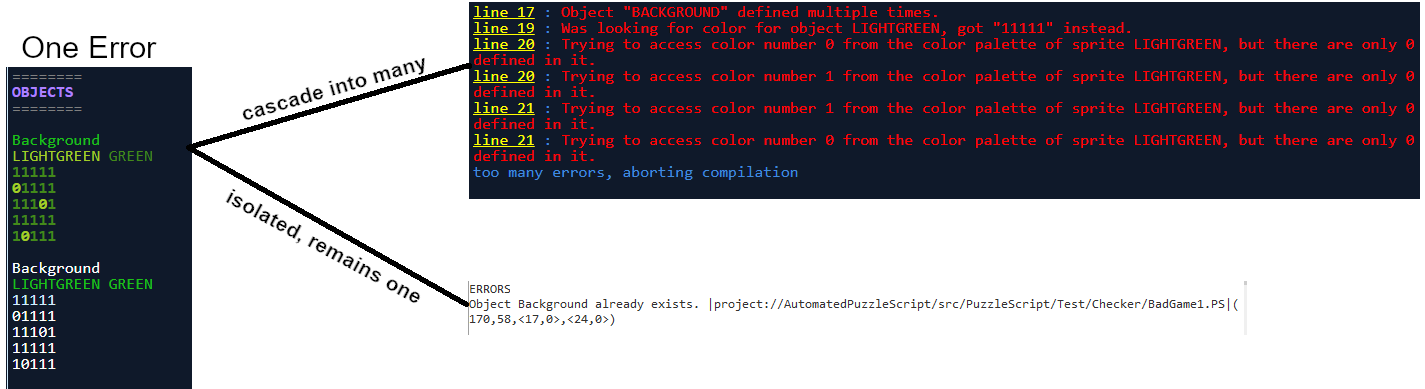
\includegraphics[width=1\textwidth]{images/Example checker.png}
    \caption{Isolation of errors}
    \label{fig:checker_example}
\end{figure}

The JavaScript implementation has 117 unique error/warning messages. This number does not account for messages that appear multiple times. Although our design currently checks for only 72 messages, the discrepancy has two reasons. As previously mentioned, using Rascal's Syntax Definition entails a certain loss of control over the feedback provided in exchange for more readability. The first reason is therefore that a part of these messages are now covered by the general parser failure error intended for the tool designer. The second reason is that, in our design, another part of the messages we extracted from the original implementation have been merged\dd. For instance, the original message has two separate messages to report on an error within the rule depending on whether that error was on the left-hand side or the right-hand side. In our design, these errors are merged into one with a keyword to differentiate the side that raised the error.

\begin{figure}[!t]
    \centering
    \begin{subfigure}{1\textwidth}
        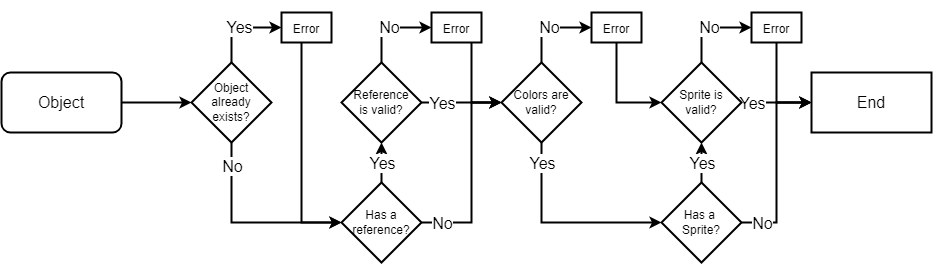
\includegraphics[scale=0.45]{images/checker/Object.png}
        \caption{Flow diagram when validating an Object}
        \label{fig:checker_object}
    \end{subfigure}
    \begin{subfigure}{1\textwidth}
        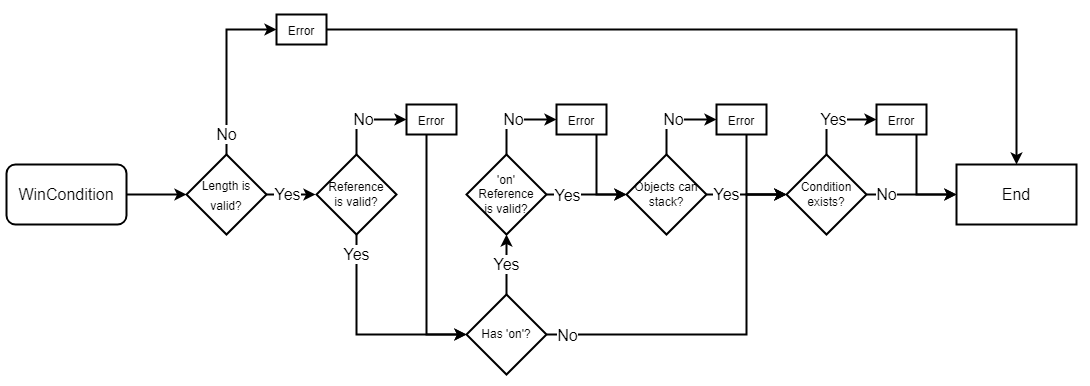
\includegraphics[scale=0.45]{images/checker/WinCondition.png}
        \caption{Flow diagram when validating a WinCondition}
        \label{fig:checker_condition}
    \end{subfigure}
    \caption{Flow diagrams illustrating the validation process done by the checker}
\end{figure}

Figure \ref{fig:checker_object} shows an example of how the checker processes a PuzzleScript component, in this case an Object. Diamonds represent tests that the checker submits the code to and rectangles represent an outcome. This is a simplification of the process that omits specifics on what is considered 'valid'. For instance, a valid color is either a HTML color code or a selection from the color palette selected by the game designer in the prelude. Objects that do not pass the requirement generate an error message that is returned by the checker, to be displayed later. In some cases, an early error causes the remaining checks to be skipped as can be seen in Figure \ref{fig:checker_condition} which illustrates the process for a Win Condition. Figure \ref{fig:checker_remaining} shows how the static checker validates the remaining components of PuzzleScript. Once detected an error is not immediately displayed but rather stored\dd, this serves the dual benefit of making it easy for the IDE to customize how they display the messages and allowing us to centralize our human-readable conversions of these messages. As a result, our redesign is easier to extend in the cases where a tool designers wants to modify the messages. For instance, if a tool designer wants to translate PuzzleScript, all they have to do is go through a single file to have access to the messages. 

In our design, error messages have several different types and subcategories. The main types are \emph{errors} and \emph{warnings}, support for lower categories exist but are currently unused. Generated messages also fall under one of a few sub-categories:
\begin{itemize}
    \item Invalid: The component's syntax is not respected making it unusable
    \item Undefined: The reference/object with that name is never defined but is used
    \item Existing:  The reference/object with that name already exists, but the code is trying to define it again. Sometimes this is generated as an error and sometimes as a warning depending on whether the engine can handle it.
    \item Unused: A warning, the code defines a reference/object/sound but never uses it\dd.
    \item Misc: Very specific errors that do not occur in enough numbers to justify a category
\end{itemize}

We categorize each error with a degree of importance based on whether or not it has a negative impact on the game and its ability to run. Error-level messages can cause issues or unintended side effects in the code that may make the game impossible to resolve, warning-level messages indicate dead or unoptimized code, and information-level messages inform the game designer on gameplay quality and possible best practices. A full list of errors and warnings raised by our tool can be seen in Appendix B. 

\begin{figure}
\vspace*{-4pt}
%\begin{minipage}{0.31\columnwidth}
%\begin{lstlisting}[language=PuzzleScript, xleftmargin=4pt]
%Background
%red green
%11111
%01111
%11101
%11111
%10111
%
%Background
%Red Green
%11111
%01111
%11101
%11111
%10111
%\end{lstlisting}
%\subcaption{duplicate object}
%\end{minipage}
%
%
\begin{minipage}{0.32\columnwidth}
%vRozen: what is Bonk?
\setulcolor{red}
\begin{lstlisting}[language=PuzzleScript, xleftmargin=2pt, , basicstyle=\ttfamily\footnotesize]
Player
black $\color{BurntOrange}orange$ $\color{darkgray}white$ $\color{blue}blue$
$\color{black}.000.$
$\color{black}.$$\color{BurntOrange}111$$\color{black}.$
$\color{darkgray}22222\ul{22222}$
$\color{black}.$$\color{blue}333$$\color{black}.$
$\color{black}.$$\color{blue}3$$\color{black}.$$\color{blue}3$$\color{black}.$
\end{lstlisting}
\setulcolor{black}
% \vspace*{-9.5pt}
\subcaption{Sprite not 5x5}
\setulcolor{black}
\end{minipage}
\hspace{12pt}
%
\begin{minipage}{0.31\columnwidth}
\setulcolor{red}
\begin{lstlisting}[language=PuzzleScript, xleftmargin=4pt,  basicstyle=\ttfamily\footnotesize]
####
#.O#$\ul{..}$
#..#$\ul{\#\#..}$
#@P.$\ul{.\#}$
#..*
#..#$\ul{\#\#}$
####$\ul{..}$
\end{lstlisting}
\subcaption{Uneven level rows}
\setulcolor{black}
\end{minipage}
\hspace{12pt}
\begin{minipage}{0.28\columnwidth}
% \setulcolor{Gold}
\begin{lstlisting}[language=PuzzleScript, xleftmargin=4pt, basicstyle=\ttfamily\footnotesize]
Crate
$\color{BurntOrange}orange$ $\color{Green}\ul{green}$
$\color{BurntOrange}00000$
$\color{BurntOrange}0$$\color{black}...$$\color{BurntOrange}0$
$\color{BurntOrange}0$$\color{black}...$$\color{BurntOrange}0$
$\color{BurntOrange}0$$\color{black}...$$\color{BurntOrange}0$
$\color{BurntOrange}00000$
\end{lstlisting}
\subcaption{Unused color}
\setulcolor{black}
\end{minipage}
\medskip

\begin{minipage}{\columnwidth}
%, xleftmargin=4pt, basicstyle=\ttfamily\scriptsize]
\setulcolor{red}
\begin{lstlisting}[language=PuzzleScript, basicstyle=\ttfamily\footnotesize]
[Eyeball| ... |Player] -> $\ul{[> Eyeball|Player]}$
\end{lstlisting}
\vspace*{-4pt}
\subcaption{Missing ellipsis in right hand side of rule}
\setulcolor{black}
\end{minipage}
\medskip

\begin{minipage}{\columnwidth}
%, xleftmargin=4pt, basicstyle=\ttfamily\scriptsize]
\setulcolor{red}
\begin{lstlisting}[language=PuzzleScript, xleftmargin=10pt, basicstyle=\ttfamily\footnotesize]
[> Player|Crate] -> [> Player] $\ul{[> Crate]}$
\end{lstlisting}
\vspace*{-4pt}
\subcaption{Unexpected rule part in right hand side of rule}
\setulcolor{black}
\end{minipage}

\caption{Errors and warnings detected by the checker}
\label{fig:ErrorsWarnings}
\vspace*{-8pt}
\end{figure}

As we previously mentioned, our tool raises errors and warnings that do not exist in the original implementation. Part of these messages are merges and others are brand news\dd. A sample of these new messages is displayed in Table \ref{tab:new_errors}. Many of these messages reference existing objects that are never used. Unused objects present two issues. The first issue is that unused objects represent dead code that inflate the file size but add no value. Dead code adds unnecessary complexity to the codebase and makes it more difficult to understand. The second issue is that unused objects may also give a false impression of the game. This false impression of the game makes it hard for other game designers to understand the design of the game. Our tool also raises a warning when redundant components are implemented into the game. For instance, duplicate win conditions can happen when game designers are not fully aware of what object a legend references. This can cause them to create duplicate instances through the use of different legends referencing the same item. Finally, ScriptButler performs additional checks on Win Conditions, an area left relatively untouched by the original implementation. We design checks to ensure that game designers do not accidentally write conditions that are mutually exclusive.

\begin{table}
\centering
\caption{New errors in ScriptButler}
\label{tab:new_errors}
\begin{tabular}{l|l|l}
Name                               & Type    & Message                                                                                                                    \\ \hline
existing\_sound                    & Warning & \begin{tabular}[c]{@{}l@{}}A sound event has already been \\ registered for this object with \\ these actions\end{tabular} \\
existing\_condition                & Warning & \begin{tabular}[c]{@{}l@{}}A victory condition similar to \\ this one already exists\end{tabular}                          \\
existing\_rule                     & Warning & \begin{tabular}[c]{@{}l@{}}A rule similar to this one already \\ exists\end{tabular}                                       \\
impossible\_condition\_unstackable & Error   & \begin{tabular}[c]{@{}l@{}}A victory condition requires items \\ existing on the same layer to stack\end{tabular}          \\
redundant\_prelude\_value          & Warning & \begin{tabular}[c]{@{}l@{}}This prelude keyword does not \\ require a value\end{tabular}                                   \\
unused\_colors                     & Warning & \begin{tabular}[c]{@{}l@{}}This object defines more colors \\ than it uses\end{tabular}                                    \\
unused\_object                     & Warning & This object is defined but never used                                                                                      \\
unused\_legend                     & Warning & This legend is defined but never used                                                                                     
\end{tabular}
\end{table}

The result of this phase is a list of messages reporting on the state of the game's code. The intent is for those messages to be passed on to the IDE and displayed to the user as shown in \ref{fig:ErrorsWarnings}. The game designer gains a complete overview of the game code and an understanding of its current flaws. Once the designer has resolved the errors, the game code is passed to he compiler. The compiler is discussed in the next section.


\subsection{Compiler}
Game languages require compilers to optimize their performance. Compilers transform the code into lower-level machine code. For PuzzleScript, this means converting the DSL into Rascal data structure. ScriptButler already does part of this task during the parsing, the compilation process completes it. The compiler transforms the existing data structures further, this increases performance but reduces readability. The new data structures do not resemble the original code at all. It may even be impossible to generate code back from the compiler because the structure is lost. For instance, the compiler resolves all references, replacing them with the list of object referenced. As a result, the original reference is lost. Our compiler is separated into three phases, representing the three sections that need to be compiled. Sounds are not compiled because they are not implemented. Objects are not compiled because our tool only requires their name. As such, we only compile three sections: Win Conditions, Levels, and Rules. All three are explained in detail below.

\subsubsection{Levels}
In PuzzleScript, game designers create 2D representations of their levels with the use of legend and aggregates. However, levels are actually 3-dimension when factoring in the collision layer. As a result, we compile the levels into 3D arrays. The design decision we have to take is in which order to arrange the array and their relation to the coordinates. Each object on a level has an XYZ coordinate. X represents the row, Y the column, and Z the layer they are present on. Each of these triples is unique. We have two choices, we can either store the levels as a XYZ array or as a ZXY array. A XYZ array is an array where the first dimension represents the X coordinate, the second the Y coordinate and the third the Z coordinate. An XYZ array has a similar concept but in a different order. The order matters depending on how we match the rules. We decided on an ZXY\dd design, where the first dimension is the layer. This makes it easier to build the level layer by layer. Using the other method would allow us to build levels one row at a time but makes it harder to check using our rule system.

Levels are designed to be able to function standalone. Each level stores all the data required to function. Only the rules and win conditions are required to run a level. However, to render a level, the engine also provides access to the object sprite even if it does not use it currently. During compilation, references and aggregation are resolved and a background layer is generated for rendering purposes. The data structure makes it possible for the engine to store the contents of a level in a simple structure.

\subsubsection{Win Conditions}
Compiling win conditions is a simple process. We resolve references and store them in data structure that makes it easier to check against the 3D structures representing our levels. Levels are also compiled in a way that allows the engine to check for their contents efficiently. Because we store the contents of a level in a simple structure, we can easily check the prerequisites of certain win conditions. For instance, if a level does not contain any instance of ObjectX then the condition \texttt{'No ObjectX on ObjectY'}. This helps performance as it does not require us to go through the level pixel by pixel. The engine can simply access the list of objects contained in the level and make assumptions based on that. However, if there is an instance of ObjectX present, we then have to conduct the more expensive check.

\subsubsection{Rules}
Rules are the most complex part of PuzzleScript and we aim to simplify them in ScriptButler. This goal means that we aim to make the system simpler to extend and we make the rules simpler to debug from a game designer perspective. To this end, we leverage a feature of PuzzleScript called Abstract Patterns\footnote{\url{https://tutor.rascal-mpl.org/Rascal/Patterns/Abstract/Abstract.html}}\dd. Abstract Patterns can be used to match the code with patterns. We use it to match data structure representing a level. However, Rascal does not have native support for creating these Abstract Patterns. The patterns are intended to be used statically to match specific code patterns. We need to be able to generate Abstract Patterns from the Rules written by game designers. We achieve this by generating Abstract Patterns as code to be interpreted by our engine\dd. This design decision incurs a performance loss, as the Rascal code is not compiled but interpreted.

Figure \ref{fig:Rule Compilation Code} shows a simple Rule written in PuzzleScript. This rule allows the player to push a crate. Using our compiler, we transform the rule into a Rascal Abstract pattern that can be seen in \ref{fig:Rule Compilation Pattern}. The pattern represents a 3D array similarly to the compiled form of a Level. In this instance, the game has three layers, as such the first dimension of the array is three elements long. However, the objects referenced in the original layer only exist on the third layer. As such, the first two layers (lines 2 and 3) match for anything and then pass the match to the replacement, changing nothing. Line 4 and 5 unpack the second and third dimension of the level, ensuring that whatever comes after and before the match is passed to the replacements pattern. Finally, lines 6 and 7 handle the actual matching. Line 7 matches a player moving in a direction and Line 8 matches a crate standing still. A similar pattern is used to replace the crate with a moving crate.

\begin{figure}[!t]
    \begin{subfigure}{1\textwidth}
        \begin{lstlisting}[language=rascal]    
        1 # [ 
        2 #     [ *layer0 ], 
        3 #     [ *layer1 ], 
        4 #     [ *prefix_lines2, 
        5 #         [ *prefix_objects2, 
        6 #             Object player0 : moving_object(str name0_0_2 : /player/, int id0_0_2, str direction0_0_2 : relative_right, Coords coords0_0_2 : <xcoord0, ycoord0, zcoord0_0_2>), 
        7 #             Object crate0 : object(str name1_0_2 : /crate/, int id1_0_2, Coords coords1_0_2 : <xcoord1, ycoord1, zcoord1_0_2>), 
        8 #         *suffix_objects2 ], 
        9 #     *suffix_lines2 ]
        10# ]
        \end{lstlisting}
        \vspace*{-8pt}
        \caption{An abstract pattern of the rule in Figure \ref{fig:Rule Compilation Code}}
        \label{fig:Rule Compilation Pattern}
    \end{subfigure}
    
    \begin{subfigure}{1\textwidth}
        \begin{lstlisting}[language=PuzzleScript]
        [ >  Player | Crate ] -> [  >  Player | > Crate  ]
        \end{lstlisting}
        \vspace*{-8pt}
        \caption{A simple PuzzleScript Rule allowing pushing Crates}
        \label{fig:Rule Compilation Code}
        \vspace*{-8pt}
    \end{subfigure}
    
    \caption{Compiling rules}
    \label{fig:compiling rules}
\end{figure}

The compiler requires multiple passes to compile a rule into a list of abstract patterns. However, the end result is more readable from the perspective of a tool designer. Our aim with this design decision is to make it easier to extend PuzzleScript with additional features in rules. Validating Abstract Patterns is easier than validating functions like the original implementation generates. 

The result of the compiler is a list of data structures for Win Conditions, Rules and Levels which can be run by the engine. The data structures we compile are easier to extend than the original implementation. This decision does not change anything for the game designer besides a performance impact caused by the new design focus on extensibility and maintainability. 

\subsection{Engine}
We divide the game loop into additional phases to avoid unnecessary coupling. We make it so that the phases only require the necessary data to be passed\dd, as opposed to passing the entire game. Figure \ref{fig:engine_flow} shows a full flow diagram of the engine, we briefly explain the different phases below:
\begin{itemize}
    \item Plan Move: Mark player objects as needing to be moved if the player has given a move command
    \item Apply Rules: Apply the rules as many times as possible
    \item Do Move: Move all objects marked as such, if there is an obstacle, see if we can move that obstacle
    \item Apply Late Rule: Apply the late rules as many times as possible.
    \item Check Victory: Check if we meet all the victory conditions, if not, do the loop again
\end{itemize}

The engine provides support to the game loop in the form of individual functions\dd. The game loop we design uses those function to run the game. We made this design decision to make it simple for other developers to create their own version of the loop by assembling the functions in a different order. Tool developers can also override the function to inject their changes without modifying the loop. For avoiding infinite loops, users can specify a limit on the number of times a rule can be applied.

\begin{figure}[!t]
    \centering
    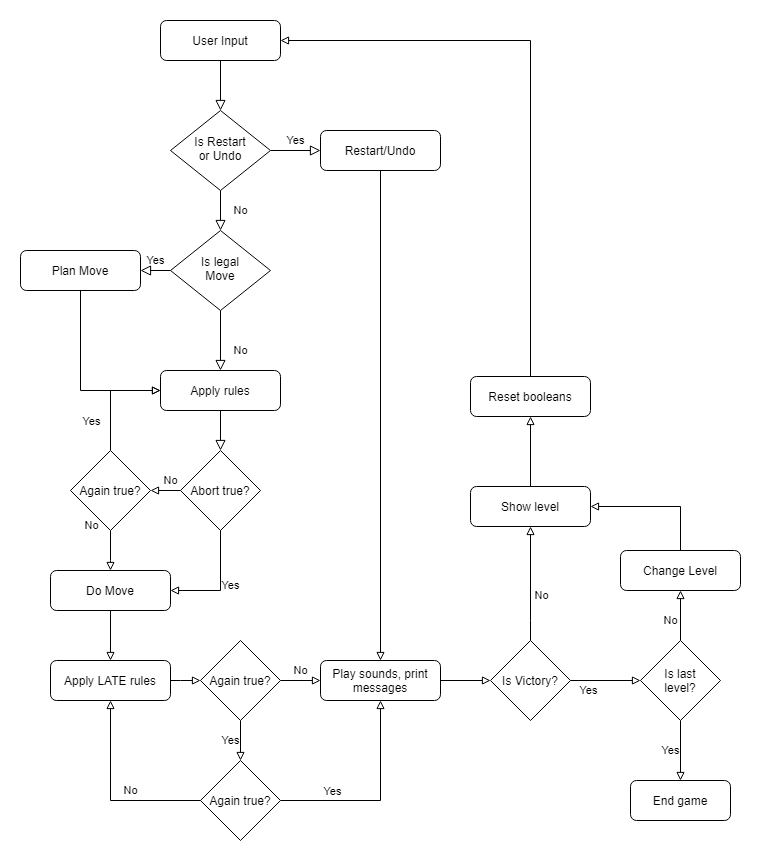
\includegraphics[width=1\textwidth]{images/Engine Flow.drawio.png}
    \caption{Engine flow graph}
    \label{fig:engine_flow}
\end{figure}



\section{Extending our implementation}
We extend the design of our PuzzleScript implementation with several features to support iterative game design. First, we design a dynamic analyzer that provides the game designers with feedback on their gameplay. Second, we implement a plugin that provides syntax highlighting and error reporting within Eclipse. Finally, we design a user-facing interface using Salix to run games. Below, we detail these functionalities one by one. 

\subsection{Dynamic Analyzer}
Our dynamic analyzer phase runs after the engine phase, allowing game designers to gather gameplay-related feedback. The phase runs subsets of the compiled code in the background when the project is built. This process is more expensive than a static check but not required as often. Messages are generated the same way as the static checker and can be manipulated similarly by IDEs.

We perform two types of dynamic analysis, standard dynamic analysis that checks for general gameplay quality and "trivial solutions". The standard dynamic analysis either checks components individually or by seeing how a few different ones interact together. Our "trivial solutions" follow in the line of thinking of our original questions on the complexity of finding fun. Finding a solution to a level is similarly complex, checking if a level can be solved is more of an AI question. Our design makes it possible to implement an AI plugin to solve this problem but that is not the focus of this thesis. Therefore, instead of trying to determine if a game is fun by checking if a level is solvable in an interesting way, we make check whether a game could be unfun by checking if a level is solvable using uninteresting solutions.

Currently, two trivial solutions exist:
\begin{itemize}
    \item Unidirectional: Is it possible to win the level by only going in one direction
    \item Unruled: Is it possible to win the level without using any rules.
\end{itemize}

\textbf{Unidirectional} is done by running a level in the background with the four directional inputs. If after submitting the length of level times two in inputs the level is not won then it is not considered \textbf{unidirectional} in that direction. If none of the four inputs come up positive, the level passes. For \textbf{unruled}, we use the compiled version of Levels and WinConditions to check whether all objects required are present on the map. This does not, however, check if they are reachable, simply whether they are present or not. 

When performing our standard dynamic check, we verify the following:
\begin{itemize}
    \item Instant Victory: Is the win condition already fulfilled for the level before player interaction
    \item Impossible Victory: Does the win condition require objects that are not present and not supplied by any rules
    \item Rule Similarity: A deeper check where we compare the compiled forms of the rules to see if they are similar
    \item Metrics: We provide various metrics to the game designer that might be useful. This data is provided without analysis to avoid possible misinterpretation. 
    \item Unusable Rule: Similarly to Impossible Victory, we check whether the prerequisites for a rule can be spawned by another rule. 
\end{itemize}

Our dynamic analysis is done similarly to our static checking, it is its own phase, but instead of taking an AST of the game, it takes a compiled engine. The same maintainability and extensibility principles apply as with the rest of the tool. Adding more dynamic checks is a simple matter of writing the logic, adding messages and calling the logic from the main function. The result is also similar, a list of messages to be manipulated as the tool designer desires. The common next step is to display those messages in the IDE.

\subsection{IDE}
\label{sec:ide}
% Explain how we integrated our language to IDE, don't make it too much of a big deal though since it only works with Eclipse. 
ScriptButler offers an IDE plugin integrated within Eclipse. This plugin leverages the fact that Rascal's Eclipse integration. Using simple code we add an outline, syntax coloring, a contextual menu, and log messages. We aim to support game designers by providing more features than the IDE from the original implementation. As a reminder, the original implementation provides syntax coloring and partial error reports. Additionally, it also provides features that allow game designers to share and export their games. However, we specifically focus on tools that provide support for game designers in their explanation of the design space.

The first feature that ScriptButler's IDE provides is syntax coloring. This feature already exists within the original implementation. In our design, we tie it to the parse tree annotations\dd. Users can change the coloring without having to change the code of the grammar or mess around with regular patterns. Additionally, this decision is important because the annotations are generated dynamically during the post-processing phase. Syntax coloring improves readability and provides context to the code\cite{DBLP:conf/ppig/Sarkar15a}. Additionally, in the case of PuzzleScript we color the sprites to provide game designers with a preview of the sprite's appearance.

% \begin{figure}[!t]
%     \centering
%     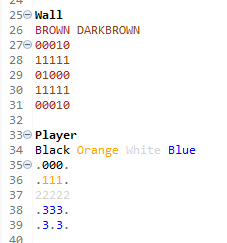
\includegraphics[width=0.50\textwidth]{images/Syntax_colouring.png}
%     \caption{Syntax highlighting}
%     \label{fig:ide_colouring}
% \end{figure}

The second feature is an outline view\dd. An outline view is a separate window the game designer can open to gain an overview of their game's contents. This feature allows the game designer to quickly navigate the file based on its contents. For instance, if a designer desires to return to the code for a specific object, they can simply click on that object's name in the outline. The outline improves the efficiency of the designer, especially as the file size grows. The outline we design provides an overview and a navigation shortcut for all major components of PuzzleScript. Tool designers can easily extend this outline to provide an overview of smaller components or to display additional data. Figure\ref{fig:ide_outline} shows this outline view with all branches expanded.

\begin{figure}[!t]
    \centering
    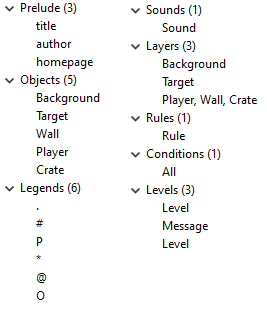
\includegraphics[width=0.5\textwidth]{images/Example_outline.png}
    \caption{IDE Outline}
    \label{fig:ide_outline}
\end{figure}

The third feature of the IDE is the display of error messages. In the original implementation, messages just appear in the console after compilation. However, this kind of implementation does not scale well with high number of messages. As such, we design ScriptButler's IDE so that it display the error messages right next to the code line creating the issue. Figure \ref{fig:ide_messages} shows this design implemented. The final feature of the IDE is a contextual menu. This contextual menu provides game designers with the ability to start up the Web GUI straight from the editor. However, the feature is very extensible and can be used for a wide variety of actions. For instance, it should be possible to use it to export the game or share it online. 

\begin{figure}[!t]
    \centering
    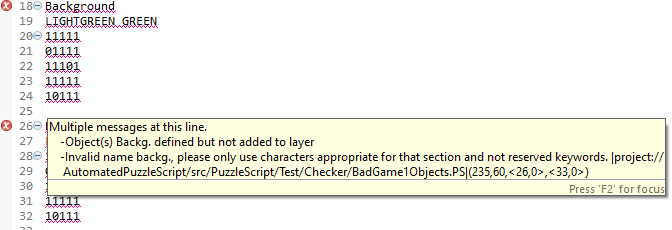
\includegraphics[width=0.85\textwidth]{images/Rascal_IDE.png}
    \caption{IDE Messages}
    \label{fig:ide_messages}
\end{figure}


In conclusion, ScriptButler's IDE provides game designers with an editor to interact with the tool itself. This editor supports game designers with a wide variety of features that make programming more efficient.




\subsection{Running Games}
ScriptButler offers game designers the ability to run their game in a browser. In the original implementation, this feature is coupled with the editor. However, we separate it and extend its capabilities to provide playtesting support using a \emph{salix} web app. At its heart, the salix web app provides game designers the ability to run their game and to see it graphically represented through a Web GUI. We use the Web GUI because Rascal does not possess the feature to represent the game graphically or to 'wait' for user input. We leverage this weakness as a strength by also extending the Web GUI with useful playtesting tools. 

The GUI provides a list of victory conditions and whether or not they are true in the current level state. Game designers can use this feature to check their assumptions of what their victory conditions are. They can create a level state where they think certain conditions should be true and then check whether or not they actually are. The GUI also provides a list of rules, how many times they were used in the last turn and what they look like when compiled. The last part is probably more useful to engine developers, which is why it's hidden from sight by default. Game designers can use this feature to check whether the rules actually run when they intend them to, and how many times they match. Finally, the GUI provides game designers with a \emph{'layered'} view of their level. A 'layered' view is a representation of the level where objects are separated based on which collision layer they appear on. This feature provides an easy way for users to see all objects on a particular pixel that may otherwise be hidden by objects they are stacked under.

The Web GUI provides tool to support the game designers when they debug their games. It uses salix which means it is, for a majority, written in Rascal. This design decision makes it easier to edit for those seeking to modify or extend the tool. The downside to our approach is that salix is still a relatively new library and suffers in regard to response times. Figure \ref{fig:salix_webserver} shows an example of Web GUI's appearance. 

\begin{figure}[!t]
    \centering
    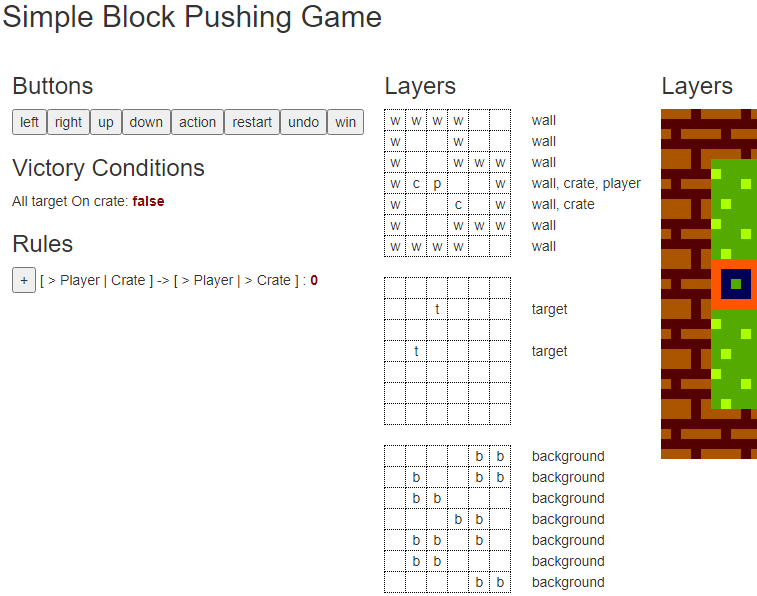
\includegraphics[width=1\textwidth]{images/Rascal Salix.png}
    \caption{Salix web app}
    \label{fig:salix_webserver}
\end{figure}
\section{Testing}
\label{sec:testing}
%  Explain unit tests conducted in this project
Here we describe an extensive test suite that verifies ScriptButtler's implementation works according to its design. We describe how the suite tests different parts of the tool and what the test results are. We validate and verify our tool using two separate methods. We describe validation Chapter \ref{ch:case} and verification in this chapter. The test suite consists of a dozen sections that test each section of our PuzzleScript implementation. The tests can be found on the GitHub repository\footnote{\url{https://github.com/ClementJ18/Rascal-PuzzleScript/tree/main/src/PuzzleScript/Test}}.

Each section consists of several PuzzleScript files containing mock data and one Rascal file that conducts the tests. The test files are intended to either verify correctness or error handling. Verifying correctness consists of running valid code through the section we are testing. Verifying error consists of running invalid code and testing to see if a controlled error message is raised. The test files consist of mock data which represent games, sections and atomic components of PuzzleScript. The complexity of the mock data varies based on the test requirements.

\paragraph{Parser}
The test suite verifying the Parsing phase is the most extensive but also has the simplest mocking data. We test individual elements of a game such as objects, rules parts and levels; complete sections and full games. We test for the correctness of this phase by checking whether or not our grammar successfully parses the mock data. Conducting additional tests to verify the integrity of the parsed data during this phase is unnecessary, the data is verified in future phases. In the cases where the parsed data is invalid, then the Abstract Syntax Tree (AST) itself will raise an error, therefore, we verify the parsed data in the phase where we verify the AST. We reuse the mock data from the parsing test suite quite frequently as mock data for our other test suites. 


\paragraph{Static Checker}
The next suite performs verification on the functionality of the static checker by purposefully triggering errors. The mock data consists of sections of PuzzleScript games plus a few additional cases that do not fit in any particular section. Throughout our test suite, we also have mock data which specifically focus on getting a correct result, and this mock data is used both for verification and to guide us during development.

\paragraph{Test-Driven Development}
Our approach to development is test-driven, so we develop by designing tests first and then writing code that passes those tests. Test-driven development requires the test suite to be designed with intent. We focus on creating tests that provide coverage for both high-level and low-level functions.  The test suite grows in complexity as it progresses through the phases of compilation. The time running the suite takes also increases as the tests run increasingly more code. Running tests for the dynamic analysis phase is the most expensive currently.

\paragraph{Results}
Running our tests gives us feedback on the quality of our tool's source code. ScriptButler is able to parse and statically check the majority of valid source code with an insignificant amount of incorrect error reporting. However, the tool struggles when it has to parse code that has severe structural issues. This causes exception in the runtime of the tool usually resulting in a crash. There is no application with native support for counting of code lines in Rascal. However, we can use \emph{cloc} and count it as if it was Java code to get an estimate. The core of our PuzzleScript implementation totals 9 files and 2317 lines of code. As a reminder, PuzzleScript's official implementation had 3 core files that totaled 5820 lines of code. In Table \ref{tab:test_suite_results} we show the number of tests associated with each section and the percentage of those tests that pass. Note that some tests are used in multiple phases. If a phase does not have any test files, then that means it reuses mock data from previous phases.

\begin{table}
\centering
\caption{Results of our test suite}
\label{tab:test_suite_results}
\begin{tabular}{l|l|l|l|l}
Phase            & \# of test files & \# of tests & Tests passed & Comments                                                                                               \\ \hline
Parser           & 28               & 28          & 24/28        & \begin{tabular}[c]{@{}l@{}}Failing tests all relate to \\ comment parsing\end{tabular}                 \\
Post-processing  & 0                & 16          & 15/16        & \begin{tabular}[c]{@{}l@{}}Failing test relates to comment \\ parsing\end{tabular}                    \\
Checker          & 9                & 9           & 9/9          &                                                                                                        \\
Compiler         & 0                & 0           & 0/0          & \begin{tabular}[c]{@{}l@{}}Verified through the engine \\ behavior\end{tabular}                       \\
Engine           & 11               & 12          & 10/12        & \begin{tabular}[c]{@{}l@{}}Advanced games do not properly \\ run\end{tabular}                          \\
Dynamic Analyser & 7                & 6           &              &                                                                                                        \\
IDE              & 1                & 1           & 1/1          &                                                                                                        \\
Interface        & 0                & 1           & 1/1          &                                                                                                        \\
Comment Parsing  & 7                & 7           & 6/7          & \begin{tabular}[c]{@{}l@{}}Tests are relatively simple, not\\ representative of all cases\end{tabular} \\
General Parsing  & 83               & 1           & 72/83        & \begin{tabular}[c]{@{}l@{}}Only tests whether games parse, \\ no data validation\end{tabular}              
\end{tabular}
\end{table}


\begin{figure}[ht]
    \label{fig:checker_remaining}
    \begin{subfigure}{1\textwidth}
        \centering
        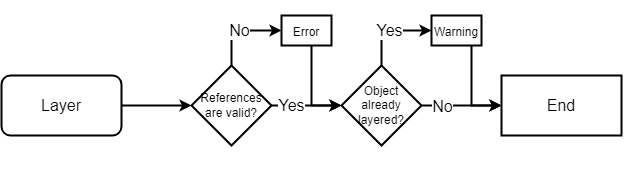
\includegraphics[scale=0.45]{images/checker/Layer.png}
        \caption{Flow diagram when validating a Layer}
    \end{subfigure}
    \begin{subfigure}{1\textwidth}
        \centering
        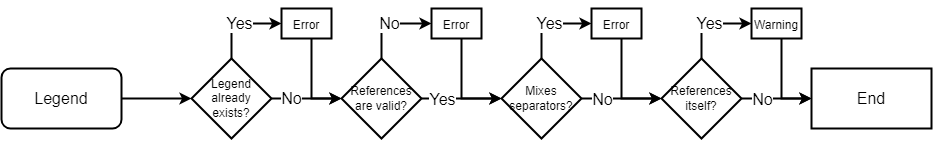
\includegraphics[scale=0.45]{images/checker/Legend.png}
        \caption{Flow diagram when validating a Legend}
    \end{subfigure}
    \begin{subfigure}{1\textwidth}
        \centering
        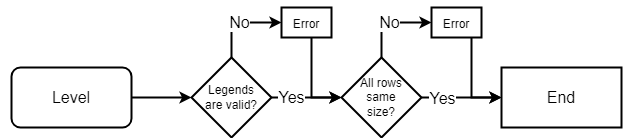
\includegraphics[scale=0.45]{images/checker/Level.png}
        \caption{Flow diagram when validating a Level}
    \end{subfigure}
    \begin{subfigure}{1\textwidth}
        \centering
        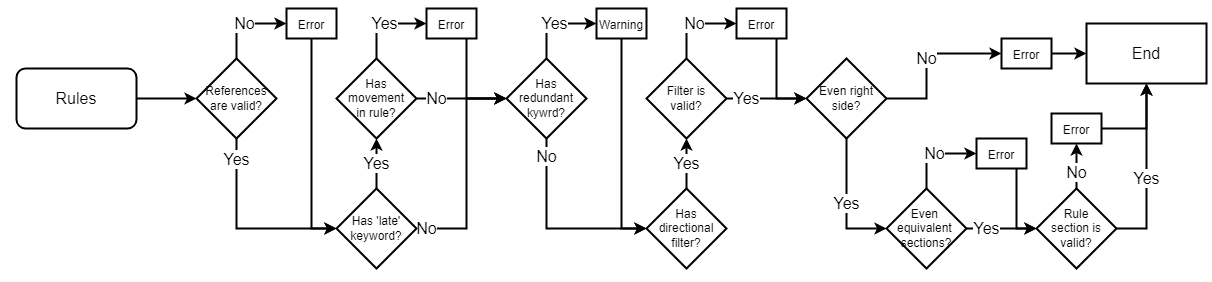
\includegraphics[scale=0.55]{images/checker/Rule.png}
        \caption{Flow diagram when validating a Rule}
    \end{subfigure}
    \begin{subfigure}{1\textwidth}
        \centering
        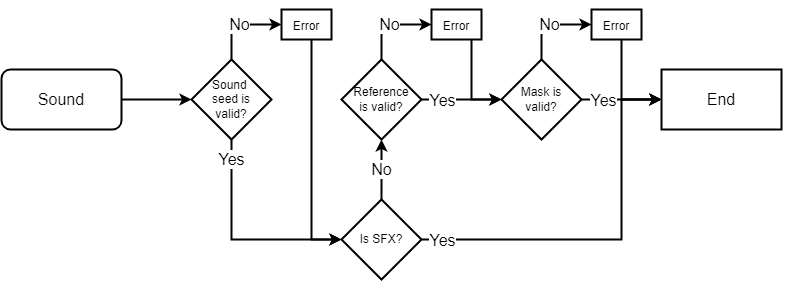
\includegraphics[scale=0.45]{images/checker/Sound.png}
        \caption{Flow diagram when validating a Sound}
    \end{subfigure}
    \caption{Flow diagrams for checker validation.}
\end{figure}
\chapter{Case Study}
\label{ch:case}
% INTRODUCTION
% concise introduction to the chapter, its goals, and structure.
In this chapter, we discuss the case study we conducted in order to validate our prototype tool, ScriptButler. The goal of a case study is to demonstrate that the functionality of our tool actually answers our research questions. We previously verified our tool in Section \ref{sec:testing} and in this chapter, we validate it. 

We first describe the game we chose for our game study, what kind of game it is, what kind of features it has and why it is useful for our purpose. We then explain the methodology we use when conducting our case study and what kind of results we expect. We explain what the results are designed to show. Finally, we describe our actual results, reflect on them and discuss how they prove the validity of the tool.

The reason that we do this case study on an existing game rather than designing our own specifically for a case study is that we do not have game designers as part of the project team. This means that any game we created would not be created by the target audience of the prototype tool. 


% The chapter is broken down as follows:
% \begin{itemize}
%     \item We describe the game we selected for the case study, what kind of features it has, how it works and why we selected it.
%     \item We describe the methodology that we use when conducting our case study and what kind of results we expect. We also describe what our results are designed to show.
%     \item Finally we describe our results, reflect on them and discuss how they prove the validity of our tool.
%     \item 
% \end{itemize}

\section{Methodology}
% describe the measurements and tests, and what they are designed to show.
Our case study is based on the following hypothesis:\newline
\quad \textit{"If we remove specific parts of the code then the game should still compile and run but the gameplay should \emph{break}."}

\textit{Break} is defined as issues indirectly caused by the removal of certain code. For example, removing a game mechanic that allows players to push a crate has the direct effect of making it impossible for the player to push a crate. However, it also has the indirect effect of making levels where pushing crates is required impossible to solve. This is because removing code also has a direct effect on gameplay and how the player can interact with the game, functionality is related to gameplay. 

Game designers create their game iteratively, as such, code is bound to be removed and added as the software evolves. We simulate this iterative by removing code from the game based on the impact it will have and observing how the tool reacts. We create three modified versions of the game, each of the modification change a single line of code but creates a large impact on the gameplay. The modifications are all listed in Table \ref{fig:case_study_experiment} and explained below.

% each version has a small modification, an expected goal and an objective. The objective is meant to describe what we expect the result to prove as far as validation goes. The three modifications, their expect results and objectives can be seen in Figure \ref{fig:case_study_experiment} and explained below.

Please note that we do not test our prototype tool on the published version of the game but on our own modified version, even in the case when we test on an "unmodified" version. This modified version includes additional newlines and the removal of redundant white space so as to make it simpler for our prototype grammar to parse it efficiently. Line numbers used in this chapter all reference lines in our modified versions which can be found on the repository of the project\footnote{\url{https://github.com/ClementJ18/ScriptButler/tree/main/src/PuzzleScript/Test/Case}}

% Our first modification is the removal of line 210, which is the win condition that states that no object Objective must be present. 

The first modification removes the win condition, which states that no object must be present (line 210). As previously explained this is intended to be the first part of every level, with the second part being the return to the Exit objects. The Win Conditions are one of the three main parts of a game where software evolution can have heavy indirect consequences. The other two that we will be testing in this case study are Game Mechanics (Rules) and Level Layouts (Levels).

Modifying win conditions changes how the player interacts with the levels, large parts of the intended player routes are made optional, changing the difficulty rating and obstacles that the player faces. The error messages that appear are used to make sure the game designer realizes that so that they can take the appropriate steps. In this case, the appropriate state, given that the removal of the win condition is intended, is to restructure the level so that the player needs to avoid guards to reach the exit.

\begin{figure}[!t]
    \centering
    \caption{Experimental setup}
    \begin{tabular}{p{4cm}|p{11cm}}
    \textbf{Action} & \textbf{Expected Results} \\ \hline
    Remove the "No Objective" win condition & Tool should raise errors due to levels that can be completed without user interaction or by going in a single direction \\ \hline
    Remove rule \#2 & Tool should raise errors stating that a win condition is impossible because there is no way to get meet it given that it is not already fulfilled on a level \\ \hline
    Remove Exit objects from levels & Tool should raise an error stating the level is impossible because there is no way to get from the current level set up to a level setup that meets the win conditions \\ \hline
    \end{tabular}
    \label{fig:case_study_experiment_old}
\end{figure}

% The second modification is the removal of the rule on line 193, this rule allows the player to remove the Objective object, fulfilling the requirement of "No Objective".

The second modification is the removal on the rule that allows the player to remove the Objective object (line 193). This rule is the mechanic that allows players to satisfy the "No Object" win condition. Removing the rule should remove the mechanic and therefore make it impossible to satisfy the condition. Theoretically, this should only apply to levels where there is an Objective present to remove but in the case of this game, it is every level. Even in the case where it doesn't actually apply to any level the tool assumes that win conditions are intended to be fulfilled on at least one level. If that is not the case, then another error is raised stating the condition is already fulfilled, which alerts the game designer to the problem. This modification relates to how the change in source code changes game mechanics and impact player interaction.

The third modification we perform is the removal of all Exit objects from certain levels, hence making these levels impossible to solve because of the evolution of level layouts. When level layouts evolve it sometimes causes the level to become unwinnable or to simply become too easy to win. Because the game only has two victory conditions and one of them is a negation we can only check this by removing the Exit objects. Removing other objects will have either no effect or will cause pathfinding issues which our prototype tool does not check for.

All three modifications are extreme cases of software evolution, the case in which something is removed. These cases are meant to illustrate how iterative design can render break gameplay or render it redundant and how meta-programming tools can help solve the problem. The results of the experiments are error and warning messages generated by our prototype and attached directly to the IDE at the appropriate line.

\section{Timothy's Adventure}
% describe the case of Timothy's adventure. What is the game and how does it work.
The game we are studying, Timothy's Adventure has a simple concept. Steal the shiny objective, avoid the guards and escape. You cannot escape until you have stolen the shiny objective.

The victory conditions are expressed in two lines, that state the objective must have been removed and that the player must be on the "exit" tiles. The narrative of this game is that the player is some sort of thief who must grab some shiny object (represented as the objective) and exit the room (by being on the exit objects). As with most PuzzleScript games, a lot of its mechanics and defeat/victory conditions are implied and must be discovered by the user, usually either through the use of common design choices or through messages at the beginning of the level.

For this case study, we extracted the exact win conditions and game mechanics by observing the code. There are five key mechanics defined by about a dozen rules. The first is tied to the \textit{Objective} Win Condition, it states that if a player is near an Objective object and presses the action key it replaces it with another object, removing that specific Objective from being an obstacle for the condition. The next two mechanics relate to the defeat condition of the game. PuzzleScript does not provide the ability to create defeat conditions the same way it provides for victory conditions. By default, the defeat condition is a softlock, an event that happens when player interaction reaches a level state that cannot become a level state that meets the conditions even if the player can still alter the level. Sometimes, as with this particular game, the designers create explicit defeat conditions with rules that automatically restart the level if the player reaches a certain state. Two mechanics take care of this defeat condition, the first one states that if a Guard object is on the same X or Y axis as the Player object then they will move one block in the player's direction and the second states that if a Guard is adjacent to the Player object then the Player object is replaced with another object representing that the player got "caught" and then the level restart at the next loop.

\begin{figure}[!t]
    \centering
    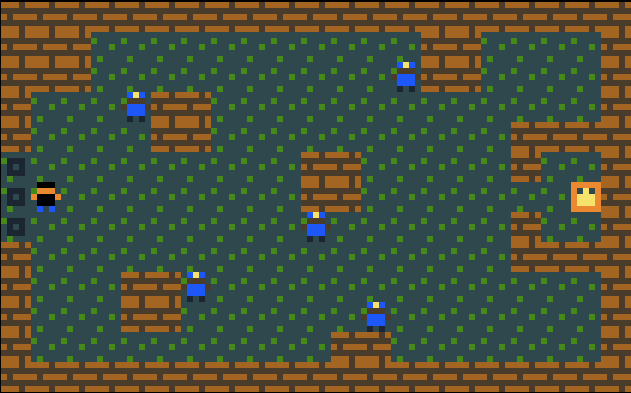
\includegraphics[width=0.75\textwidth]{images/case_results/Case_game.png}
    \caption{A level from the case game showcasing the general layout with the exit on the left, the objective on the right and the guards in blue}
    \label{fig:case_game_example_old}
\end{figure}

Finally, the game has two mechanics which represent tools that the players can use to solve certain levels. The first mechanic, introduced in level 5, allows the player to step on a Button object which transforms every Door object on the same X and Y axis into a different object which neither the player nor the guards can go through. This is usually used to stop guards from getting to the player but can also softlock the player if used without care. The second mechanic and the most complex one of the game is related to movement. It states that if the player steps on a Portal object then they will be teleported to the equivalent portal object on the same X or Y axis given that it is not obstructed. This is used to allow the player to move to rooms that are not connected to one another or to escape guards as they cannot use the portal.

% There are five game mechanics expressed in about a dozen rules:
% \begin{itemize}
%     \item Pressing action next to the switch flips it
%     \item Being on the same X or Y axis as a guard makes them move towards you
%     \item Being adjacent to a guard on the start of the turn makes you lose the level
%     \item Stepping on a button activates all the walls on the same X or Y coordinate
%     \item Stepping on a portal sends you to a portal if one exists unobstructed on the same X or Y coordinate
% \end{itemize}

The game contains 14 levels, each of them created with the goal of gradually increasing the difficulty by introducing new challenges and new mechanics to solve those challenges. 

\section{Results}
% you describe the experimental results, and you reflect on them.
Here we validate ScriptButler in a case study of the game called Timothy's adventure.
% Without modifications, our prototype tool raises the following errors and warnings, by order of appearance:

We first run the tool on an unmodified version of the game to see what errors or warnings may already exist and find the following issues, by order of appearance:
\begin{itemize}
    \item WARNING: Line 33 - Color \textbf{white} not used in object Background 4
    \item WARNING: Line 161 - Legend \textbf{ + } defined but not used
    \item WARNING: Line 199 - Right side of rule similar to rule on line 200
    \item WARNING: Line 200 - Right side of rule similar to rule on line 199
    \item ERROR: Line 202 - Objects in section need to be able to stack but appear on the same layer.
\end{itemize}

We first want to address the error, a false positive as a result of a misinterpretation of PuzzleScript's design. The side of the rule with the error is \texttt{Background no Wall no Door\_on}, which the checker interprets as meaning that the three items specified should be able to stack when in fact what this line actually means is that there should be no wall or door present on this background.

There is an argument to be made there that this is an unnecessary ambiguity since when objects are aligned in a part of the rule it usually means that they should be able to stack. In addition, there are already tools that can avoid this sort of ambiguity by creating an extra \textbf{or} reference that include both, as can be seen in Figure \ref{fig:case_ambiguity}

\begin{figure}[!t]
\begin{lstlisting}[language=PuzzleScript]
Obstacle = Wall or Door_on
[> Temp Teleport | Background no Obstacle] -> [ Teleport > Player_stealth | Background]
\end{lstlisting}
\vspace*{-8pt}
\caption{Removing design ambiguity from the rule}
\label{fig:case_ambiguity_old}
\vspace*{-8pt}
\end{figure}

The remaining warnings are all valid but not critical as they are mainly dead code or intended false positives that inform designers about potential issues with gameplay.

\subsection{Modifying Victory Conditions}
\textit{Remove the ”No Objective” win condition}

The results of the modification matched our expectations, removing the win conditions labelled all the levels are trivially solvable by going in a single direction. This modification theoretically matches our idea of rapid feedback but, in practice, our prototype implementation cannot identify trivial solutions fast enough to be considered rapid feedback. This is caused by optimization issues with the engine and not with the dynamic analyser, as such, optimization work on the engine will easily resolve our issue with performance in the dynamic analysis. A sample of the warning messages generated next to the levels can be seen in Figure \ref{fig:modification_1_results}

\begin{figure}[!t]
    \centering
    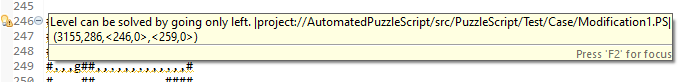
\includegraphics[width=1\textwidth]{images/case_results/Modification_1_Results.png}
    \caption{Warning messages are shown after applying modification 1}
    \label{fig:modification_1_results_old}
\end{figure}

\subsection{Modifying Game Mechanics}
\textit{Remove rule \#2}

The result of the modification matched our expectations, removing the first rule triggered a warning stating that the win condition "No Objective" is now impossible to fulfil, given that it is not already fulfilled on a level. The tool assumed by default that every rule and every win condition is used on every level, this means that some of the messages are false but those can simply be ignored by the game designer. Guessing whether or not a rule is intended to be used by the game designer could lead to a lot of false negatives. We prefer having some false positives that the designer can ignore rather than false negatives that they may never find out about.

The error message can be seen in Figure \ref{fig:modification_2_results}, it is located on the same line as the problematic win condition although it does hide it when hovered as can be seen on this screenshot. As a reminder, our tool does not conduct any pathfinding analysis as this is more of an AI-focused goal. We assume that the player is able to reach the necessary objects for victory and focus on whether or not they are able to interact with them in a way that could lead to a solution. 

\begin{figure}[!t]
    \centering
    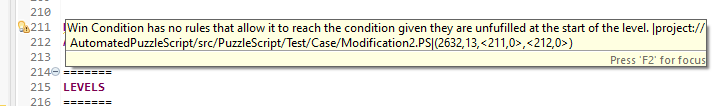
\includegraphics[width=1\textwidth]{images/case_results/Modification_2_Results.png}
    \caption{A warning message is shown after applying modification 2}
    \label{fig:modification_2_results_old}
\end{figure}

\subsection{Modifying Level Layouts}
\textit{Remove Exit objects from levels}

This case study was trickier than we initially intended. Player objects have special rules attached to them related to their movement and as such the tool needs to be specifically told that the object has those special rules. The rest is simple enough, analyse if the object is present on the map, if it is not, analyse if there is a way to spawn it. Because of the special rules we do not need to perform this analysis on the players, our assumption is that at least one player object is always present 

For every condition not already met on a level, we check if it can be met specifically within the context of this level. As with others, this can lead to false positives, especially with complex levels in which conditions only become an obstacle to victory after a prerequisite has been met. Although these cases are rare as this usually means that this prerequisite has to be filled anyways in order to reach the condition. 

\begin{figure}[!t]
    \centering
    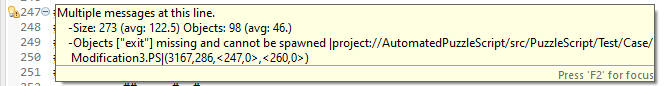
\includegraphics[width=1\textwidth]{images/case_results/Modification_3_Results.png}
    \caption{A warning message is shown after applying modification 3}
    \label{fig:modification_3_results_old}
\end{figure}

\begin{figure}[!t]
\begin{lstlisting}[language=PuzzleScript]
(BEFORE)
###########
#....O....#
#.........#
#.........#
#.........#
#....P....#
####EEE####

(AFTER)
###########
#....O....#
#.........#
#.........#
#.........#
#....P....#
####...####
\end{lstlisting}
\vspace*{-8pt}
\caption{Removing exit objects from level}
\label{fig:case_m3_modification_old}
\vspace*{-8pt}
\end{figure}

We validated this check by temporarily adding a rule to the modification that would allow the player to spawn an exit. This successfully erased all error messages relating to that issue.

\section{Conclusion}
In our case study, we set out to show that the error and warning messages that ScriptButler raises are indeed related to the software evolution in games and that the tool can indeed tell the game designer when their code changes impact the gameplay in a negative manner. 

We use simple examples to answer our hypothesis since these simple examples can easily be confirmed by playing the game manually to validate them. Therefore, since we know that our examples are valid cases of software evolution impacting gameplay in a negative way, we can validate our tool by having the tool raise warnings on the cases.

It accomplishes the goal for all three of the modifications from which we can then extrapolate, with a small degree of incertitude related to validity threats (discussed in Section \ref{sec:threats}), that our tool could accomplish the same with more complex cases of software evolution having an impact on gameplay. 

% \section{Threats to validity}
% % What could affect the validity of your research? Think of pitfalls of your research method, experimental setup, interpreting the results.

% Our prototype tool does suffer from a few issues but the core of it is functional. The two main threats to the validity of our results is performance and feature-completion.

% We, however, not do perceive these as critical threats to the validity of our research. We have proven that we are able to implement a bit of everything that PuzzleScript offers and we have found no reason to believe that the rest would be impossible to implement. Making the engine feature complete will be complex but not impossible. 

% Performance is a more complicated issue. A large part of the performance issue comes from an initially shaky understanding of PuzzleScript's design. Our understanding became more solid as the project progressed which allowed us to fix some of the issues. The first step to fixing performance would most likely make the tool feature complete first once the every part of the implementation is done it would be easier to understand how to rework the code to make it more optimal.




\chapter{Discussion}
\label{ch:discussion}
In this chapter, we discuss the results of our project.

\section{Design Formalization}
Our first contribution is a document outlining the syntax of a PuzzleScript file. We studied PuzzleScript's design by observing how the games behaved under various inputs and by going through the codebase. Based on this we created a document containing details on the design of PuzzleScript and the conclusion of our observations. This document is Chapter \ref{ch:puzzlescript} of the thesis. The aim of the document was to create documentation on the syntax structure of PuzzleScript so that we could parse it using a formal grammar. The document is complete enough for others to create their own parser and documents the corner cases of PuzzleScript. It lays out the basic constraints that certain objects must abide by. For all the constraints of PuzzleScript, refer to Appendix A.

\section{ScriptButler}
We then used our formalization of PuzzleScript's design to create our own design of an implementation which we then implemented. Our goal was to create a more extensible and maintainable implementation of PuzzleScript. This prototype is not a feature-complete implementation of PuzzleScript as can be seen in Table \ref{fig:feature_comparison}. However, it is complete enough to provide feedback on a wide range of games. This range includes published games.

\begin{figure}[!t]
    \centering
    \caption{Feature Comparison between the original implementation and our implementation.}
\begin{tabular}{l|l|l|l}
    \textbf{Category} & \textbf{Feature}           & \textbf{JavaScript} & \textbf{Rascal}       \\ \hline
    \textit{Editor}   & Text Editor       & Yes                       & Yes                         \\
             & Syntax Coloring   & Yes                       & Yes                         \\
             & Messages          & No                        & Yes                         \\
             & Game frame        & Yes                       & Yes                         \\
             & Autocomplete      & Yes                       & No                         \\
             & Export            & Yes                       & No                          \\
             & Share             & Yes                       & No                          \\
             & Save states       & Yes                       & No                          \\
             & Keyboard control  & Yes                       & Yes                         \\
             & Debug             & Yes                       & Yes, more extensive         \\
    \textit{Parser}   & Error Checking    & Yes                       & Yes, generic error          \\
             & Grammar           & Implicit                  & Formal                      \\
    \textit{Checker}  & Error Checking    & N/A                       & Yes                         \\
             & Errors            & 101                       & 72                          \\
             & Warnings          & 19                        & 11                          \\
             & Error Isolation   & No, cascades              & Yes                         \\
    \textit{Compiler} & Error Checking    & Yes                       & None                        \\
             & Prelude           & Implemented               & Implemented up to Checking  \\
             & Objects           & Implemented               & Implemented                 \\
             & Legend            & Implemented               & Implemented                 \\
             & Sounds            & Implemented               & Implemented up to Checking  \\
             & Layers            & Implemented               & Implemented                 \\
             & Rules             & Implemented               & Implemented, mostly working \\
             & Win Conditions    & Implemented               & Implemented                 \\
             & Levels            & Implemented               & Implemented                 \\
    \textit{Engine}   & Randomness        & Implemented               & Implemented                 \\
             & Rigid Bodies      & Implemented               & Not Implemented             \\
             & Real time         & Implemented               & Not Implemented             \\
             & Rule Loops        & Implemented               & Not Implemented             \\
    \end{tabular}
    \label{fig:feature_comparison}
\end{figure}


The grammar we created using our design document can parse most games, but it struggles with parsing comments. Currently, we strip the comments before parsing similarly to the JavaScript implementation. In the future, parsing comments could prove an interesting source for metrics. Ultimately, the grammar is a very literal representation of a PuzzleScript file that can be easily extended and modified to alter PuzzleScript's design. The static checker is fully functional but does not currently check for the errors of the original implementation. This is an intentional design decision, we instead focused on implementing new types of errors within our checker that the original implementation did not check for. There are no obstacles to reimplementing all the error messages but they did not provide a lot of value for this project. The compiler and engine work on a wide range of simple games. We do not currently implement complex features such as real-time or rigid bodies. These features are complex to implement and not commonly used in games. We design and implement the engine as a collection of plugins that can easily be exchanged. This design decision should make it easier to optimize in the future.

The final result is a partial reimplementation of the PuzzleScript engine. This implementation can run most simple games, is more extensible and more maintainable than the JavaScript one. We achieve this by reducing the coupling and code density. We leveraged Rascal features to make the compiled Rules more readable and verify the functionality using the extensive test suite discussed in \ref{sec:testing}.

\section{Supporting Game Designers}
To support game designers, we implemented three additional components into our tool: 1) an IDE, 2) an interface for running games and playtesting, and 3) a dynamic analyzer for automated gameplay testing.

The IDE allows game designers to edit their games, similarly to the in-browser editor of the original JavaScript implementation. It provides syntax coloring, an outline, a contextual menu and displays error messages. The IDE allows designers to access the feedback generated by ScriptButler in a user-friendly way as it directly attaches it next to the problematic line. We provide several other features that the original editor does not provide. However, we do not support the extra features that the original editor had such as the ability to share the game on GitHub or to export it as an HTML page. The reason is that does features do not have an impact on game quality. The only feature from the current editor we would potentially look at reimplementing is the 'Rebuild' feature. This feature re-compiles the game while it is running, allowing changes to game mechanics, victory conditions, and object appearance to take effect immediately. 

The interface implements the ability for designers to run and play their games. This component was separated from the IDE, unlike the original implementation, so that we could expand it. The interface provides the game designers with tools that can be used to debug their game. An important difference between our implementation and the original's is that our editor does not use keyboard buttons but rather requires the player to click on UI buttons. This error should be fixed in future works when salix supports keyboard events. Future works could also split the interface between the 'game designer view' and the 'tool developer view' to enhance the purposes of both.

Finally, the dynamic analyzer is similar to the static checker. It generates error messages that are then processed by the IDEs and displayed to game designers. However, the messages relate to the quality of the gameplay rather than the quality of the code. The dynamic analyzer provides the game designer with feedback on the playability of their game. In terms of playtesting, this feedback is shallow. However, we purposefully keep the feedback shallow so that we can provide it rapidly, it is an intentional design decision.


\section{Research Questions}
Here we discuss how our work contributes to answering our research questions. We begin by discussing the subquestions and then we describe how they help us answer our main research question.

%\textbf{RQ1.1}: How can PuzzleScript be used for studying game mechanics?
\subsection{RQ1.1} 
As we have discussed previously, PuzzleScript rules are very closely tied to the affordances they provide players. The match and replace patterns almost literally define game mechanics. This simplification allows us to more easily study the effect of code changes on game mechanics. We show this in the dynamic analyzer of ScriptButler. When the game designer removes a piece of code, the tool provides feedback on how it impacts the game mechanics required to solve certain levels or meet certain victory conditions. Despite being relatively simple, PuzzleScript is a powerful and popular game language. This popularity ensures that we study features that meet game designer's need. We could study a programming language, this would make the code easier to analyze. However, studying a programming language does not represent a realistic scenario. Game designers use game engines, so we have to study a game engine.

\subsection{RQ1.2} 
When iteratively designing, game developers evolve the software of their game over time, sometimes causing changes with a negative impact on the quality of gameplay. Game designers can reduce the impact of these changes by putting in place mitigation strategies such as playtesting. 

These strategies are time-consuming and unreliable. Playtesting requires a human to play through the entire game and actively attempt to break it. Sometimes, AI can be used to automatically play through the game and try to detect gameplay issues. However, this presents the same issue of how incredibly time-consuming this approach is, both in terms of time investment in putting together an AI that can play a game and having the AI test the game. Therefore, the game designers put in place tests to verify gameplay. These tests work similar to unit tests, they provide an input to the game and expect an output. This output is usually a specific game state. These tests allow for automated game design. However, the tests need to be adapted as the requirements change, creating additional dependencies. The tests can only be created within the context of a specific game and cannot be generally applied to a game engine.

\subsection{RQ1}
% \textbf{RQ1}: How can meta-programming tools and techniques be used to empower PuzzleScript game designers and allow them to freely explore the design space of their game?
We now know how PuzzleScript code relates to the code and why that relation is useful. We know strategies that game designers can put in place to mitigate the negative effects of software evolution. Therefore, we now apply meta-programming techniques to implement these mitigation strategies by leveraging the connection between code and game mechanics. 

We propose a system of solutions that can be generally applied to any game written using PuzzleScript. These tests provide rapid feedback in a live programming context. Instead of having to run a long test suite, the tool responds live to changes and provides the designer feedback live. This system of solutions is implemented as a tool, called ScriptButler. The tool is more efficient than a player because it does not require a full game. With only a few lines of code, it can already start providing feedback on the game.

We note that this does not make human testers redundant. Human testers are much better are detecting defects with the visual aspect of the game. Humans are more creative,  they can break the game in more interesting ways. Although the extensible nature of our tool means that if new, general ways of breaking game are discovered, they can be incorporated. Finally, humans actually experience the game as a whole and can provide feedback on that experience. Our tool simply tests a few interconnected components. ScriptButler empowers game designers by reducing their dependence on playtesting. The playtesters can then focus on the testing more complex problems that actually relate to the way humans experience a game. 

\section{Threats To Validity}
\label{sec:threats}
\paragraph{Game Designer Involvement}
No game designers were actually involved in the process of creating our tools, but we still want our tools to be useful to game designers. This is a threat to validity in that we were not specifically told by game designers that the issues we identified are indeed issues. Instead, we relied on data we gathered from personal experience and from observing the evolution of PuzzleScript games. We mitigate this as much as possible by grounding our research using a case study. The case study mimics scenarios of realistic software evolution. We apply ScriptButler to those scenarios to see to what extent the feedback provided evaluates the impact of those changes. Since the case is simple, we can also validate the errors raised by ScriptButler manually.

% method

\paragraph{Reverse Engineering}
Reverse engineering is not a perfect method for extracting a design from source code. This is illustrated in our case study where we misinterpreted the observed behavior causing an error that does not actually happen in the JavaScript implementation. This error happens because we did not specifically test for this kind of behavior when reverse-engineering the engine. We partially mitigated this issue by conducting extensive testing on our engine using published games, which we first checked against the original PuzzleScript engine. However, this method is not completely reliable since we also try to test for new types of errors within our implementation.

\paragraph{Incomplete Engine}
Our implementation of PuzzleScript does not cover all the features of the original implementation. As such, there is a possibility that the features that remain unimplemented cannot be implemented using Rascal. However, we strongly believe that this will not occur as we have successfully implemented rules, the most complex PuzzleScript features. 

% and as such believe that it will also be possible to implement other functionality such as rigid bodies and loops.

\paragraph{Academic Prototype}
ScriptButler is an academic prototype. Additional work is required to make the tool suitable for professional work. However, ScriptButler has sufficient feature coverage to be used within the context of our project. We needed an extendable implementation of PuzzleScript which allowed us to run PuzzleScript games and perform dynamic analysis on them and the tool met that need. If the tool was required to meet the needs of professional game developers, work would have to go into optimizing the engine and covering the remaining corner cases. Additionally, the formal grammar we have created is still unable to parse more complex combinations of lexicals, especially when combined with code that is heavily commented. Future work should look into making it possible to parse comments as they may contain interesting possible metrics to judge code and gameplay quality\cite{TAN2015493}.


\chapter{Related work}
\label{ch:related_work}
Here we discuss works related to our project.

\section{Automated Game Design}
In this section, we discuss the various works that are related to the automated game design aspect of our project. First, we go over projects that have similar goals to ScriptButler and contrast the differences. In the last section, we delve into the AI perspective of AGD. This perspective is not the focus of our thesis, but it is an important part of AGD.

\subsection{AI-Based Automation}
AI-Based automation is used in two distinct ways in Game Design and we will briefly discuss each. We do not discuss AIs as part of a game but rather AI as a tool for game design and development. Although AI as part of games is an interesting area as they provide additional replayability and randomness to a game. That perspective was briefly covered in our Procedural Content Generation section.

The first way that AI-based automation is used is as a way to support developers in their endeavors through such things as automated mechanics testing. Automated mechanics testing is similar to playtesting in that a player goes through the level insuring that certain actions result in certain level states. However, the method does not provide the ability to analyze the experience. AI-based playtesting is a relatively new area of game design that involves both physical games\cite{10.1145/3102071.3102105} and digital games. The concept is having an algorithm crawl the game's various obstacles and come up with solutions much more methodically than a human could.

The second way that AI-based automation is used is as a way to support the designers in their endeavors through such things as AI-generated content. This can include things like automatically generating levels based on game mechanics, generating game mechanics based on a preset, or generating a narrative based on rules. In these cases, the AI system influences the mechanics and aesthetics of the game. Game design provides context to the AI which in turn generates affordances for the game based on the domain of the game as can be seen in Figure \ref{fig:ai-based game design}.

\begin{figure}[!t]
    \centering
    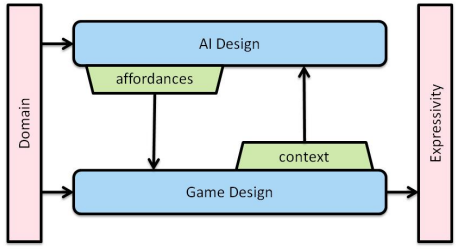
\includegraphics[width=0.66\textwidth]{images/AI-based game desig.png}
    \caption{Illustrating the process of AI-based game design (adapted from Eladhari\cite{Eladhari2011AIBasedGD})}
    \label{fig:ai-based game design}
\end{figure}

This concept is well illustrated in the paper by Eladhari\cite{Eladhari2011AIBasedGD} which discusses the concepts of context and affordances before relating them to the iterative design loop. Another paper by Eladhari\cite{10.1145/1501750.1501798} discusses a technical framework called \textit{Mind Module} which aims to model emotion in the world of games. This module generates parts of the game based on the player responses.

\subsection{Examples of AGD}
\paragraph{PlaySpecs} A paper by Osborn et al.\cite{osborn2015playspecs} connects the concepts of automated analysis with software verification. This is similar to our approach where we apply techniques used in software engineering to perform automated game analysis. The author proposes the tool \emph{Playspecs} to test PuzzleScript games. Any puzzle game can define Playspecs conditions that must hold for any found solution on each level. A solution that violates this constraint notifies the developer. However, PlaySpecs requires play traces to analyze. In the paper, this is done by generating solutions using a heuristic search. In other cases, this could be also done manually through playtesting. PlaySpecs' target audience is game engines and engine developers.

\paragraph{Ludoscope} Dormans proposes the tool \emph{Ludoscope} as a way to analyze how level space relates to level missions. They illustrate those concepts in "Adventures in level design"\cite{DBLP:conf/fdg/Dormans10} in the context of a \emph{The Legend of Zelda} game. Ludoscope is a general-purpose tool for generating content using transformational grammars. Ludoscope is extensible and in a validation follow-up validation experiment by Dormans\cite{Dormans2013CombinatorialAE}. The tool can then be extended based on project-specific needs. Ludoscope touches on the concepts of automated game design and procedural content generation. Game designers define constraints for generation and the tool provides feedback after the generation. ScriptButler does not generate any content but it is similarly extensible. 

\paragraph{Micro-Machinations} \emph{Micro-Machinations}\cite{DBLP:conf/sle/KlintR13} (MM) is a textual and visual programming language that extends \emph{Machinations}. Van Rozen and Dorman\cite{DBLP:conf/fdg/RozenD14} propose a live programming approach as an embeddable MM library. This approach of rapid prototyping is similar to our approach with ScripButler. However, our approach does not focus on providing alternative methods for creating those games, only feedback on existing code.



\section{PuzzleScript}
PuzzleScript's popularity and features generate a lot of interest for developers looking to research game design. Because of that, a few other works have been done relating to it. In this section, we present these different works and how they relate to our project.

We want to mention the project by GitHub user vexorian\cite{puzzlescript-bfs} which implements Breath-First search as a PuzzleScript game. It does not necessarily relate to this project but shows an interesting way of applying Puzzlescript in education. Users can create their own levels to test how breath-first search interacts with it and study the Rules of the game to understand how it works in theory. 

The project repository recommends running the project on a fork of PuzzleScript which includes additional features\footnote{\url{https://pancelor.com/PuzzleScript/editor.html}} such as the ability to jump to specific levels. It is another of those forks that extend PuzzleScript with very small specific changes to suit their needs\cite{pancelor}.

\subsection{Other Implementations}
Here we compare the features of different implementations of PuzzleScript which we previously discussed in Section \ref{ch:background}. The comparison can be seen in Table \ref{fig:feature_comparison_rw}. The bottom line is that none of these implementations really focus on changing the design process of PuzzleScript game, they are all focused on simply reimplementing PuzzleScript in a different language for convenience. The Rust implementation specifically mentions that it handles rules differently from the original engine but that seems to cause issues. We did not compare PatternScript\cite{PatternScript} because it is an implementation of PuzzleScript in JavaScript, something we already knew possible since the original implementation is in JavaScript.

\begin{figure}[!t]
    \centering
    \caption{Feature Comparison between the original implementation and other implementations.}
\begin{tabular}{p{2cm}|p{3cm}|p{2cm}|p{2cm}|p{2cm}|p{2cm}}
\small
    \textbf{Category} & \textbf{Feature}    & \textbf{JavaScript}   & \textbf{C++}                 & \textbf{Rust}           & \textbf{C}                    \\ \hline
    \textit{Editor}   & Text Editor         & Yes                   & No                           & No                      & No                            \\
                      & Syntax Coloring     & Yes                   & No                           & No                      & No                            \\
                      & Messages            & No                    & No                           & No                      & No                            \\
                      & Game frame          & Yes                   & No                           & No                      & No                            \\
                      & Autocomplete        & Yes                   & No                           & No                      & No                            \\
                      & Export              & Yes                   & No                           & No                      & No                            \\
                      & Share               & Yes                   & No                           & No                      & No                            \\
                      & Save states         & Yes                   & No                           & No                      & No                            \\
                      & Keyboard control    & Yes                   & No                           & Yes                     & Yes                           \\
                      & Debug               & Yes                   & No                           & No                      & No                            \\
    \textit{Parser}   & Error Checking      & Yes                   & Yes                          & Yes                     & Yes                           \\
                      & Grammar             & Implicit              & Implicit                     & No, JSON-based          & Implicit                      \\
    \textit{Checker}  & Error Checking      & N/A                   & N/A                          & No                      & Yes but no line number        \\
                      & Errors              & 101                   & 101                          & N/A                     & 101                           \\
                      & Warnings            & 19                    & 19                           & N/A                     & 19                            \\
                      & Error Isolation     & No, cascades          & No, cascades                 & N/A                     & No                            \\
    \textit{Compiler} & Error Checking      & Yes                   & Yes                          & N/A                     & Yes                           \\
                      & Prelude             & Yes                   & Mostly missing               & Yes                     & Yes                           \\
                      & Objects             & Yes                   & Implemented                  & Yes                     & Yes                           \\
                      & Legend              & Yes                   & Implemented                  & Yes                     & Yes                           \\
                      & Sounds              & Yes                   & No                           & Yes                     & No                            \\
                      & Layers              & Yes                   & Yes                          & Yes                     & Yes                           \\
                      & Rules               & Yes                   & Yes, commands missing   & Yes                     & Yes, mostly working           \\
                      & Win Conditions      & Yes                   & Yes                          & Yes                     & Yes                           \\
                      & Levels              & Yes                   & Yes                          & Yes                     & Yes                           \\
    \textit{Engine}   & Randomness          & Yes                   & No                           & Yes                     & Yes                           \\
                      & Rigid Bodies        & Yes                   & No                           & Yes                     & No                            \\
                      & Real time           & Yes                   & No                           & Yes                     & Yes                           \\
                      & Rule Loops          & Yes                   & No                           & Yes                     & No                            \\
    \end{tabular}
    \label{fig:feature_comparison_rw}
\end{figure}

\subsection{Solvers}
Here we discuss how solving algorithms are used in PuzzleScript. We have found three instances of AI being applied to PuzzleScript with the purpose of automated playthrough.

A paper by Chong-U Lim and D. Fox Harrell\cite{6932896}\footnote{\url{https://github.com/icelabMIT/PuzzleScriptAI}} present a repository with a series of algorithms for solving PuzzleScript levels. However, the most interesting part is that the project is not simply implementing an AI but provides an interface for anyone to implement their own algorithms. The similarity between this paper and our own project is interesting, except that instead of providing a wrapper for PuzzleScript we provide our own implementation with its own endpoints. A project by Lauren Cunningham\cite{PuzzleScriptSolver} uses the extension to implement a Monte Carlo Tree Search and shows how exactly one can use such tools. 

A project hosted by GitHub user marcosdon\cite{PuzzleScriptWithSolver} is a full PuzzleScript editor and as such is very easy to play around with. The project adds a "Solve" button to the top bar which runs through the level extremely fast and provides a series of movements to solve the level. It only provides one solution, however, so when there are multiple ways to solve a level, it should be interesting to see which one it picks. The interface uses PuzzleScript's code but the algorithm itself is quite simple, as such it gets easily stuck. We tested on the game we selected for our case study and it became essentially stuck at the third level, always getting caught by the guards. Perhaps it needs more PuzzleScript-specific awareness. This is where the previous project is useful as it allows users to extend the algorithms themselves.




\chapter{Conclusion}
\label{ch:conclusion}

In this thesis, we have posed the question of how we could support game designers by leveraging meta-programming techniques. The solution we have proposed to address this question is a system of solution for relating gameplay and code. To implement this system, we have documented PuzzleScript design in order to simplify the creation of our own implementation. This extensive documentation of PuzzleScript's design is the first contribution of our thesis. The document details the the syntax of a PuzzleScript file enabling the creation of a parser. This document also goes thoroughly into the corner cases of PuzzleScript's syntax.

We have used our documentation of PuzzleScript's design to design our own implementation. We have addressed the technical obstacles that we faced when trying to use an existing implementation by leveraging good software engineering practices to make the implementation more maintainable and extensible. The result is the second contribution of our thesis: a general-use tool, ScriptButler, for parsing, running, and analyzing PuzzleScript games.  We have implemented our system of solutions for dynamic analysis into ScriptButler. This implementation allows game developers to get live feedback on the impact of their software changes on gameplay. We have also further extended ScriptButler with IDE support and a debugging interface.

We conclude that relating game code and game mechanics is a valuable way of providing feedback to game designers. We present ScriptButler as a tool for exploring that relation that leverages meta-programming. We believe there is much left to discover and we hope that others can extend the tool to conduct similar research by leveraging PuzzleScript.

\section{Future work}
\label{sec:future_work}
Of course, our work can be extended and improved in several ways. We discuss several directions for future work.

\subsection{Level Solver}
Our tool has been designed with the goal of leveraging meta-programming principles in the context of Automated Game Design (AGD). The approach we have focused on separating from the current AI-based approaches to AGD. However, our tool is not closed to the possibility of combining meta-programming and AI, as such, future work could look into the possibility of adding level solvers as a way of conducting a more thorough gameplay analysis as a complement to our rapid-but-shallow approach.

ScriptButler already exposes the necessary endpoints for an automated player, so the technical requirements for coupling one with the tool are quite low. This would be mostly a research endeavor, understanding how AI can fit in our concept of rapid feedback. Playtesting the entire game on every build would not be viable, so work would have to be done in understanding how the game can be broken down into parts and then executed based on the quality of feedback provided.

\subsection{Procedural Content Generation}
ScripButler transforms PuzzleScript code into Rascal data structures. Future works could extend the tool to make it possible to generate PuzzleScript code from the Rascal data structures. As such, ScriptButler could be used from a PCG perspective to study PuzzleScript. The goal of such a project could be try and generate individual levels or rules that build up into a working game. 

Levels and rules generated by future works could also be evaluated using our existing dynamic analysis module. If a level can be solved trivially, this could detected by the tool. Other trivial solutions might also arise from generating the wide range of content, improving the tool's analysis capabilities.

\subsection{Audio-Visual Research}
Part of a game's quality is how it looks and sound. This a facet of game design that we did not touch upon in this project. However, there is room to apply research in that area to our tool. For instance, some combinations of colors create contrasts that are painful to the eye. What if our tool could detect such an instance and provide a warning.

However, such a project would first have to understand how graphics and sounds interact within game design. With a few lines of code, a plugin could be added to ScriptButler to allow for such analysis.

% \subsection{Defining Fun}

\subsection{Automated Game Design for Serious Games}
Serious games are more complex to design than regular games because they have an educational component\cite{DBLP:conf/dagstuhl/BraadZS15}. PuzzleScript games can potentially be used in an educational context. We have found a game that demonstrates how breath-first search behaves using a PuzzleScript game\cite{puzzlescript-bfs}. It is not completely clear whether this is an effective method of teaching as PuzzleScript games require more intuition than most other games to play. This is one of the weaker future works, but we wanted to introduce it anyways.

% \subsection{Applying to other languages}


\chapter*{Acknowledgements}
When I first started on this project I was not sure where I was going. I knew I wanted to do something with video games, which have always been a personal interest of mine both from an entertainment perspective and a research perspective. 

There was an idea that slowly evolved, helped by the work of others, feedback from those around me and my own tinkering. This project has been one of the biggest undertakings of my life and I would not have managed to finish it if not for the support of my peers.

I am very grateful for the help of my supervisor, Riemer van Rozen, for pushing me into this project when I first approached him. He helped me understand what I wanted from my master project and helped me shape a project that met these desires. He met with me every week, sometimes more, for nearly a year, always asking the hard questions that forced me to leave no stone unturned.

I want to thank my family, and especially my mother who, without knowing anything about meta-programming, never stopped asking me questions on my work in an unorthodox variant of rubber ducking.

I also want to thank Georgia Samaritaki and Youri Reijne, the two other students supervised by Riemer. Their feedback when we discussed our projects was very helpful.

\nocite{*}
\printbibliography[type=article,title={Articles}]
\printbibliography[type=software,title={Software}]
\printglossaries%

%TC:ignore
\chapter{Appendix}
\label{ch:appendix}

\section{Appendix A}
This is a collection of errors that the JavaScript implementation of PuzzleScript raises. These were used in our project to reverse-engineering PuzzleScript's design. The messages that appear below are ripped straight from the JavaScript code. We have, however, removed duplicate messages. We wanted to centralize the messages for future works and to have an easy reference to them.

\subsection{Errors}
\begin{enumerate}
    \item "'random' cannot be matched on the left-hand side, it can only appear on the right", rule.lineNumber
    \item "A rule has to have an arrow in it.  There's no arrow here! Consider reading up about rules - you're clearly doing something weird", lineNumber
    \item "An ellipsis on the left must be matched by one in the corresponding place on the right.", rule.lineNumber
    \item "An ellipsis on the right must be matched by one in the corresponding place on the left.", rule.lineNumber
    \item "Background must be in a layer by itself.",state.lineNumber
    \item "Cannot define a property (using 'or') in terms of aggregates (something that uses 'and').", state.lineNumber
    \item "Cannot define an aggregate (using 'and') in terms of properties (something that uses 'or').", state.lineNumber
    \item "Commands should only appear at the end of rules, not in or before the pattern-detection/-replacement sections.", lineNumber
    \item "Error, an \item can only have one direction/action at a time, but you're looking for several at once!", lineNumber
    \item "Expecting sfx data, instead found "" + seed + "".", lineNumber
    \item "Got caught looping lots in a rule group :O",ruleGroup[0].lineNumber,true
    \item "Movements cannot appear in late rules.", lineNumber
    \item "Need have to have matching number of  'startLoop' and 'endLoop' loop points."
    \item "No collision layers defined.  All objects need to be in collision layers."
    \item "Oops!  " + object\_name.toUpperCase() + " not assigned to a layer.", rule.lineNumber
    \item "Something bad's happening in the LEGEND", state.lineNumber
    \item "The start of a rule must consist of some number of directions (possibly 0), before the first bracket, specifying in what directions to look (with no direction specified, it applies in all four directions).  It seems you've just entered "" + token.toUpperCase() + '".', lineNumber
    \item "There can't be more than 30 rigid groups (rule groups containing rigid members).", rules[0][0][3]
    \item "There's no point in putting an ellipsis at the very start or the end of a rule", rule.lineNumber
    \item "Trying to access color number "+n+" from the color palette of sprite " +state.objects\_candname.toUpperCase()+", but there are only "+o.colors.length+" defined in it.",state.lineNumber
    \item "You can't define object " + candname.toUpperCase() + " in terms of itself!", state.lineNumber
    \item "You can't have anything in with an ellipsis. Sorry.", rule.lineNumber
    \item "You can't use two ellipses in a single cell match pattern.  If you really want to, please implement it yourself and send me a patch :) ", oldrule.lineNumber
    \item "You cannot use 'no' to exclude the aggregate object " + c.toUpperCase() + " (defined using 'AND'), only regular objects, or properties (objects defined using 'OR').  If you want to do this, you'll have to write it out yourself the long way.", lineNumber
    \item "You have an totally empty pattern on the left-hand side.  This will match *everything*.  You certainly don't want this."
    \item "a sprite cannot have more than 10 colors.  Why you would want more than 10 is beyond me.", o.lineNumber + 1
    \item "background cannot be an aggregate (declared with 'and'), it has to be a simple type, or property (declared in terms of others using 'or')."
    \item "error detected - unexpected character " + stream.peek(),state.lineNumber
    \item "error, didn't find any object called player, either in the objects section, or the legends section. there must be a player!"
    \item "got caught in an endless startloop...endloop vortex, escaping!", ruleGroup[0].lineNumber,true
    \item "have to have matching number of  'startLoop' and 'endLoop' loop points."
    \item "no layers found.",state.lineNumber
    \item "spooky ellipsis found! (should never hit this)"
    \item "too much stuff to define a sound event.", lineNumber
    \item "you have to define something to be the background"
    \item "you have to have a background layer"
    \item '"'+n+'" is an aggregate (defined using "and"), and cannot be added to a single layer because its constituent objects must be able to coexist.', state.lineNumber
    \item 'Cannot add "' + candname.toUpperCase() + '" to a collision layer; it has not been declared.', state.lineNumber
    \item 'Cannot end a rule with ellipses.', lineNumber
    \item 'Cannot reference "' + candname.toUpperCase() + '" in the LEGEND section; it has not been defined yet.', state.lineNumber
    \item 'Encountered an unexpected "->" inside square brackets.  It's used to separate states, it has no place inside them >:| .', lineNumber
    \item 'Error in win condition: "' + candword.toUpperCase() + '" is not a valid object name.', state.lineNumber
    \item 'Error, malformed cell rule - encountered a "["" before previous bracket was closed', lineNumber
    \item 'Error, malformed cell rule - was looking for cell contents, but found "' + token + '".  What am I supposed to do with this, eh, please tell me that.', lineNumber
    \item 'Error, symbol "' + ch + '" is defined using 'or', and therefore ambiguous - it cannot be used in a map. Did you mean to define it in terms of 'and'?', level[0] + j
    \item 'Error, symbol "' + ch + '", used in map, not found.', level[0] + j
    \item 'Error, when specifying a rule, the number of matches (square bracketed bits) on the left hand side of the arrow must equal the number on the right', lineNumber
    \item 'Error, you can only use "->" once in a rule; it's used to separate before and after states.', lineNumber
    \item 'Expecting the word "ON" but got "'+candword.toUpperCase()+"'.", state.lineNumber
    \item 'Identifiers cannot appear outside of square brackets in rules, only directions can.', state.lineNumber
    \item 'In a rule, each pattern to match on the left must have a corresponding pattern on the right of equal length (number of cells).', lineNumber
    \item 'In a rule, if you specify a force, it has to act on an object.', lineNumber
    \item 'Invalid character "' + ch + '" in sprite for ' + state.objects\_candname.toUpperCase(), state.lineNumber
    \item 'Invalid color specified for object "' + n + '", namely "' + o.colors[i] + '".', o.lineNumber + 1
    \item 'Key "' + ch.toUpperCase() + '" not found. Do you need to add it to the legend, or define a new object?', state.lineNumber
    \item 'MetaData "'+token+'" has no parameters.',state.lineNumber
    \item 'MetaData "'+token+'" needs a value.',state.lineNumber
    \item 'Name "' + candname.toUpperCase() + '" already in use.', state.lineNumber
    \item 'Name "' + m + '", referred to in a rule, does not exist.', state.lineNumber
    \item 'No levels found.  Add some levels!', undefined, true
    \item 'Object "' + candname.toUpperCase() + '" defined multiple times.', state.lineNumber
    \item 'Object "' + n.toUpperCase() + '" has been defined, but not assigned to a layer.', dat.lineNumber
    \item 'Object "' + target + '" not found.', lineNumber
    \item 'Object "'+n+'" has been declared to be multiple different things',state.legend\_aggregates[i].lineNumber
    \item 'Object not found with name ' + n, state.lineNumber
    \item 'Palette "' + val + '" not found, defaulting to arnecolors.', 0
    \item 'Rule matches object types that can't overlap: "' + object\_name.toUpperCase() + '" and "' + existingname.toUpperCase() + '".', rule.lineNumber
    \item 'Spooky error!  Empty line passed to rule function.', lineNumber
    \item 'Sprites must be 5 wide and 5 high.', state.lineNumber
    \item 'The "+" symbol, for joining a rule with the group of the previous rule, must be the first symbol on the line '
    \item 'The "+" symbol, for joining a rule with the group of the previous rule, needs a previous rule to be applied to.'
    \item 'This rule has a property on the right-hand side, "' + rhsPropertyRemains.toUpperCase() + "", that can't be inferred from the left-hand side.  (either for every property on the right there has to be a corresponding one on the left in the same cell, OR, if there's a single occurrence of a particular property name on the left, all properties of the same name on the right are assumed to be the same).", lineNumber
    \item 'This rule has an ambiguous movement on the right-hand side, "' + rhsAmbiguousMovementsRemain + "", that can't be inferred from the left-hand side.  (either for every ambiguous movement associated to an entity on the right there has to be a corresponding one on the left attached to the same entity, OR, if there's a single occurrence of a particular ambiguous movement on the left, all properties of the same movement attached to the same object on the right are assumed to be the same (or something like that)).", lineNumber
    \item 'This rule has some content of the form "X no X" which can never match and so the rule is getting removed during compilation.', rule.lineNumber
    \item 'This rule refers to nothing.  What the heck? :O', lineNumber
    \item 'Trying to define aggregate "' + n.toUpperCase() + '" in terms of property "' + value.toUpperCase() + '".'
    \item 'Trying to define property "' + n.toUpperCase() + '" in terms of aggregate "' + value.toUpperCase() + '".'
    \item 'Two "+"s ("append to previous rule group" symbol) applied to the same rule.', lineNumber
    \item 'Unknown junk in spritematrix for object ' + state.objects\_candname.toUpperCase() + '.', state.lineNumber
    \item 'Unrecognised stuff in the prelude.', state.lineNumber
    \item 'Unwelcome term "' + n1 + '" found in win condition. Win conditions objects have to be objects or properties (defined using "or", in terms of other properties)', lineNumber
    \item 'Was expecting a direction, instead found "' + direction + '".', lineNumber
    \item 'Was looking for color for object ' + state.objects\_candname.toUpperCase() + ', got "' + str + '" instead.', state.lineNumber
    \item 'You cannot use relative directions ("\^v<>") to indicate in which direction(s) a rule applies.  Use absolute directions indicators (Up, Down, Left, Right, Horizontal, or Vertical, for instance), or, if you want the rule to apply in all four directions, do not specify directions', lineNumber
    \item 'You need to have some objects defined'
    \item 'You want to spawn a random "' + object\_name.toUpperCase() + '", but I don't know how to do that', rule.lineNumber
    \item 'cannot assign sound events to aggregate objects (declared with "and"), only to regular objects, or properties, things defined in terms of "or" ("' + target + '").', lineNumber
    \item 'cannot duplicate sections (you tried to duplicate "' + state.section.toUpperCase() + '").', state.lineNumber
    \item 'color not specified for object "' + n + '".', o.lineNumber
    \item 'incorrect format of legend - should be one of A = B, A = B or C ( or D ...), A = B and C (and D ...)', state.lineNumber
    \item 'incorrect format of win condition.', state.lineNumber
    \item 'incorrect sound declaration.', lineNumber
    \item 'must start with section "OBJECTS"', state.lineNumber
    \item 'names cannot end with the letter "v", because it's is used as a direction.', state.lineNumber
    \item 'no such section as "' + state.section.toUpperCase() + '".', state.lineNumber
    \item 'section "' + state.section.toUpperCase() + '" is out of order, must follow  "' + sectionNames[sectionIndex - 1].toUpperCase() + '" (or it could be that the section "'+sectionNames[sectionIndex - 1].toUpperCase()+`"is just missing totally.  You have to include all section headings, even if the section itself is empty).`, state.lineNumber
    \item 'section "' + state.section.toUpperCase() + '" must be the first section', state.lineNumber
    \item 'unexpected sound token "'+candname+'".' , state.lineNumber
    \item example[0] + ' and ' + example[1] + ' can never overlap, but this rule requires that to happen.', rule.lineNumber
\end{enumerate}

\subsection{Warnings}
\begin{enumerate}
    \item "Author list too long to fit on screen, truncating to three lines.",undefined,true
    \item "Commands should only appear at the end of rules, not in or before the pattern-detection/-replacement sections.", lineNumber
    \item "Game title is too long to fit on screen, truncating to five lines.",undefined,true
    \item "Invalid syntax, ellipses should only be used within cells (square brackets).", lineNumber
    \item "Invalid syntax. Directions should be placed at the start of a rule.", lineNumber
    \item "Invalid token " + token.toUpperCase() + ". Object names should only be used within cells (square brackets).", lineNumber
    \item "Maps must be rectangular, yo (In a level, the length of each row must be the same).",state.lineNumber
    \item "Multiple closing brackets without corresponding opening brackets.  Something fishy here.  Every '[' has to be closed by a ']', and you can't nest them.", lineNumber
    \item "Sprite graphics must be 5 wide and 5 high exactly.", o.lineNumber
    \item "This rule may try to spawn a " + o1 + " with random, but also requires a " + o2 + " be here, which is on the same layer - they shouldn't be able to coexist!", rule.lineNumber
    \item "You probably meant to put a space after 'message' innit.  That's ok, I'll still interpret it as a message, but you probably want to put a space there.",state.lineNumber
    \item "throttle\_movement is designed for use in conjunction with realtime\_interval. Using it in other situations makes games gross and unresponsive, broadly speaking.  Please don't."
    \item 'A "restart" command is being triggered in the "run\_rules\_on\_level\_start" section of level creation, which would cause an infinite loop if it was actually triggered, but it's being ignored, so it's not.'
    \item 'Janky syntax.  "|" should only be used inside cell rows (the square brackety bits).', lineNumber
    \item 'Message too long to fit on screen.', level[2]
    \item 'Unknown junk in object section (possibly: sprites have to be 5 pixels wide and 5 pixels high exactly. Or maybe: the main names for objects have to be words containing only the letters a-z0.9 - if you want to call them something like ",", do it in the legend section).',state.lineNumber
    \item 'You named an object "' + candname.toUpperCase() + '", but this is a keyword. Don't do that!', state.lineNumber
\end{enumerate}

\pagebreak
\section{Appendix B}
A list of figures related to all the errors currently implemented within ScriptButler. Some of these errors are new and some are translations from the original PuzzleScript implementation.

\begin{table}[!htbp]
\centering
\caption{Invalid errors detected by the analyzer}
\label{tab:static_errors_invalid}
\scriptsize
\begin{tabular}{ll}
% \toprule
\textbf{Name} & \textbf{Description}                                                                    \\ \hline
% \midrule
invalid\_name                                       & Name does not respect the pattern rules defined for it                        \\
invalid\_color                                      & Color not found in the chosen palette                                          \\
invalid\_sound\_seed                                & Sound seed is not a valid positive int                                         \\
invalid\_sound\_verb                                & Sound verbs not recognized                                                     \\
invalid\_sprite                                     & Sprite is not 5*5                                                              \\
invalid\_level\_row                                 & Level rows are not all equal in length                                         \\
invalid\_sound\_length                              & Sound definition has too many/not enough verbs                                 \\
invalid\_condition\_length                          & Condition definition has too many/not enough verbs                             \\
invalid\_condition                                  & Combination of condition verbs not recognized                                  \\
invalid\_condition\_verb                            & Condition verbs not recognized                                                 \\
invalid\_object\_type                               & Mixed properties and aggregates in legend definition                           \\
invalid\_prelude\_key                               & Prelude keyword not recognized                                                 \\
invalid\_prelude\_value                             & Prelude value invalid for prelude keyword                                      \\
invalid\_rule\_prefix                               & Verb not valid as rule prefix                                                  \\
invalid\_rule\_command                              & Verb is not valid as a rule command                                            \\
invalid\_sound                                      & Verb is not a valid sound                                                      \\
invalid\_ellipsis\_placement                        & Ruleparts cannot start or end with ellipsis                                    \\
invalid\_ellipsis                                   & Ellipsis must be alone in the section                                          \\
invalid\_rule\_part\_size                           & Rules must have the same number of parts on each sides                         \\
invalid\_rule\_content\_size                        & Rule parts must have the same number of sections on each part                  \\
invalid\_rule\_keyword\_amount                      & Each force in a section must be applied to exactly one object                  \\
invalid\_rule\_keyword\_placement                   & Each force in a section must be applied to exactly one object                  \\
invalid\_rule\_ellipsis\_size                       & Ellipsis must be present in both parts at the same place                       \\
invalid\_rule\_movement\_late                       & Late rules cannot match for movements                                          \\
invalid\_rule\_random                               & Random keywords cannot be used on the left side                                \\
% \bottomrule
\end{tabular}
\end{table}

\begin{table}[!htbp]
\centering
\caption{Undefined errors detected by the analyzer}
\label{tab:static_errors_undefined}
\scriptsize
\begin{tabular}{ll}
% \toprule
\textbf{Name} & \textbf{Description}                                                                    \\ \hline
% \midrule
undefined\_reference                                & Reference used but never defined                                               \\
undefined\_object                                   & Object used but never defined                                                  \\
undefined\_sound\_seed                              & Sound seed does not exist                                                      \\
undefined\_sound\_mask                              & Sound mask used but never defined                                              \\
undefined\_sound\_objects                           & Object used but never defined                                                  \\
undefined\_sound                                    & Sound event used but never defined                                             \\
% \bottomrule
\end{tabular}
\end{table}

\begin{table}[!htbp]
\centering
\caption{Existing errors detected by the analyzer}
\label{tab:static_errors_existing}
\scriptsize
\begin{tabular}{ll}
% \toprule
\textbf{Name} & \textbf{Description}                                                                    \\ \hline
% \midrule
existing\_object                                    & Object has already been defined                                                \\
existing\_legend                                    & Legend has already been defined                                                \\
existing\_section                                   & Section has already been defined                                               \\
existing\_mask                                      & Mask has already been defined for this sound                                   \\
existing\_sound\_seed                               & Seed has already been defined for this sound                                   \\
existing\_sound\_object                             & Object has already been defined for this sound                                 \\
existing\_prelude\_key                              & Prelude keyword already defined                                                \\
% \bottomrule
\end{tabular}
\end{table}

\begin{table}[!htbp]
\centering
\caption{Misc errors detected by the analyzer}
\label{tab:static_errors_misc}
\scriptsize
\begin{tabular}{ll}
% \toprule
\textbf{Name} & \textbf{Description}                                                                    \\ \hline
% \midrule
mixed\_legend                                       & Legend has both 'or' and 'and'                                                 \\
mixed\_legend                                       & Property cannot use aggregates/Aggregates cannot use properties                \\
unlayered\_objects                                  & Object defined but not added to any collision layers                           \\
ambiguous\_pixel                                    & Properties cannot be used in levels                                            \\
reserved\_keyword                                   & Cannot use keyword there                                                       \\
self\_reference                                     & Legend references self                                                         \\
mask\_not\_directional                              & Direction keywords used but mask is not directional                            \\
impossible\_condition\_duplicates                   & Duplicate conditions found                                                     \\
impossible\_condition\_unstackable                  & Conditions require items that exist on the same layer to stack                 \\
missing\_prelude\_value                             & Prelude keyword requires a value                                               \\
% \bottomrule
\end{tabular}
\end{table}

\begin{table}[!htbp]
\centering
\caption{Warnings detected by the analyzer}
\label{tab:static_warnings}
\scriptsize
\begin{tabular}{ll}
% \toprule
\textbf{Name} & \textbf{Description}                                                                    \\ \hline
% \midrule
unused\_colors                                      & Color is defined for the object but never used in sprite                           \\
no\_levels                                          & No levels have been defined for the game                                       \\
message\_too\_long                                  & The message might be too long to display                                       \\
existing\_sound                                     & Sound event already registered, registering a new one                            \\
existing\_condition                                 & Similar win condition already exists                                           \\
existing\_rule                                      & Similar rule already exists                                                    \\
redundant\_prelude\_value                           & Prelude keyword does not require a value                                      \\
multilayered\_object                                & Objects appear in multiple layers                                              \\
semantic\_warning                                   & Object that needs to be on top for victory condition present in inferior layer \\
win\_keyword                                        & Win keyword in the rule makes other commands and rule parts useless                \\
% \bottomrule
\end{tabular}
\end{table}

%TC:endignore

\end{document}
